\chapter{Modelos de crescimento liderados pela demanda}
\label{CapTeorico}

\epigraph{Is it not rather odd when dealing with ``long-run problems'' to start with the assumption that all firms are always working below capacity?}{Keynes to Kalecki}


Este capítulo subsidia as discussões teóricas dos capítulos seguintes.
Para tanto, faz-se uma breve revisão da literatura dos modelos de crescimento liderados pela demanda. Apresenta a instabilidade harrodiana para então avaliar a forma que essa problemática é tratada pelas teorias heterodoxas.
Ao longo desta discussão, serão privilegiados aqueles modelos que atendem o princípio da demanda efetiva (PDE)  e replicam alguns fatos estilizados no curto-, médio- e longo-prazo.


Para atender esses objetivos, a seção \ref{SecHarrod} explicita a instabilidade de Harrod e as respostas dos modelos de Cambridge, kaleckianos e supermultiplicador sraffiano. 
Adiante, na seção \ref{Medium}, são avaliadas as alternativas existentes na literatura de crescimento que incluem gastos autônomos não criadores de capacidade produtiva.
Em seguida, na seção \ref{SecAutonomos}, é feito um levantamento bibliográfico sobre os modelos de crescimento com gastos autônomos para então investigar, na seção \ref{RevResidencial}, as formas de incluir o investimento residencial enquanto tal.
Por fim, a seção \ref{Concl1} contém as considerações finais.


\section{Instabilidade de Harrod: princípios e provocações}\label{SecHarrod}

%=============== Inicio: Ligação Harrod ============

As origens da teoria macrodinâmica devem, em grande parte, às contribuições de \textcite{harrod_essay_1939}. Tal modelo impôs importantes questões: Existe estabilidade do crescimento no longo pra\-zo? É possível equacionar o crescimento da demanda com o crescimento da capacidade produtiva? Se sim, qual variável acomoda essa adequação? A capacidade produtiva se ajusta à demanda ou o inverso? Os modelos de Cambridge, Oxford e do Supermultiplicador Sraffiano responderam essas provocações de formas distintas e serão analisados ao longo desta seção.

%Antes de prosseguir para a Equação Fundamental de Harrod, é importante retomar dois conceitos: (i) Efeito multiplicador e (ii) Princípio Acelerador. O primeiro indica que a renda é um múltiplo dos gastos autônomos enquanto o segundo estabelece que a determinação do investimento decorre das alterações na demanda (efetiva). Argumenta-se que a junção destes dois conceitos permite tratar o Princípio da Demanda Efetiva de forma dinâmica. 

Para evitar redundâncias, são apresentadas as hipóteses que permeiam as famílias de modelos aqui avaliadas. 
A presente exposição prioriza a parcimônia e, portanto, trata-se de uma economia sem relações externas e sem governo em que tanto progresso tecnológico quanto retornos crescentes de escala estão ausentes. Além do PDE, o que torna os modelos em questão consistentes
é o abandono da substitutibilidade entre capital e trabalho e, portanto, adota-se uma função de produção
\textit{à la} Leontief em que existem dois produtos potenciais: plena capacidade ($Y_K$) e pleno emprego ($Y_L$) de modo que o produto potencial ($Y_{FC}$) é determinado por:

\begin{equation}
    Y_{FC} = \min (Y_K, Y_L)
\end{equation}
Seguindo a literatura, em que o estoque capital ($K$) é o fator escasso,
\begin{equation}
\label{Oferta}
    Y_{FC} = \cdot Y_K = \frac{1}{v}K_{-1}
\end{equation}
em que $v$ é a relação técnica capital-produto. 


Considerando as hipóteses anteriores, a determinação do produto pelos componentes da demanda é obtida pela soma do consumo e investimento. Como será visto adiante, a distinção entre os modelos recairá sobre a autonomia (completa, parcial ou nula) do investimento e a existência de gastos autônomos não criadores de capacidade produtiva (denotados por $Z$). De modo a expor o problema deixado por \textcite{harrod_essay_1939}, é necessário supondo que o consumo é completamente induzido e que não existam gastos ``improdutivos'' ($Z$). Assim, o produto determinado pela demanda é dado pelo multiplicador ($\mu$):

\begin{equation}
\label{Demanda}
Y = \mu\cdot (\overline I)
\end{equation}
O princípio acelerador\footnote{Neste caso, trata-se do acelerador rígido, tal como utilizado por \textcite{harrod_essay_1939}.}, por sua vez, estabelece que a determinação do investimento decorre das alterações na demanda (efetiva), ou seja, decorre do princípio de ajuste do estoque de capital:
$$
K = v\cdot Y
$$
\begin{equation}
I = v\Delta Y
\end{equation}


%Tomando o modelo mais genérico, em que consumo é parcialmente induzido ($C$), o investimento criador de capacidade produtiva ao setor privado ($I$) possui uma parcela autônoma ($\overline I$) e outra induzida e os gasto autônomos são não nulos ($Z > 0$), obtém-se a determinação do produto pelos componentes da demanda:
%\begin{equation}
%\label{Demanda}
%    Y = C + I + Z
%\end{equation}
A questão que permeia os modelos analisados são as condições para que exista um crescimento equilibrado da demanda (Eq. \ref{Demanda}) e da capacidade produtiva (Eq. \ref{Oferta}). 
Argumenta-se que a junção destes dois conceitos permite tratar o Princípio da Demanda Efetiva de forma dinâmica e que esta é a essência do modelo de Harrod cuja Equação fundamental pode ser deduzida da identidade entre poupança ($S$) e investimento\footnote{Para o caso com acelerador rígido e uma dada propensão marginal a consumir ($c$), o consumo é induzido, tem-se:
$$
Y = c\cdot Y + v\cdot \Delta Y
$$
rearranjando, obtém-se:
$$
\frac{\Delta Y}{Y} = g = \frac{1 - c}{v} = \frac{s}{v}
$$
que equivale à equação fundamental de Harrod deduzida adiante.
}:

$$
s\cdot Y = S \equiv I
$$
Neste ponto, fica evidente que neste modelo a propensão marginal à poupar ($s$) é igual a propensão média à poupar ($S/Y$) na ausência dos gastos autônomos não criadores de capacidade\footnote{As implicações desta igualdade será analisada mais detidamente ao tratar do supermultiplicador sraffiano.}. Em seguida, basta normalizar esta identidade pelo estoque de capital,
$$
\frac{I}{K} = s\frac{Y}{K}
$$
$$
\frac{I}{K} = s\frac{Y}{v\cdot Y_K}
$$
\begin{equation}
    g_K = \frac{s}{v}u
\end{equation}
em que $g_K$ é a taxa de acumulação e $u$ é o grau de utilização da capacidade definido por:
$$
u = \frac{Y}{Y_FC}
$$
e sua taxa de crescimento pode ser dada por
$$
g_u = g_Y - g_{Y_{FC}}
$$
Além disso, para que o grau de utilização se estabilize, é preciso que, no \textit{steady state}, produto e capacidade produtiva cresçam a uma mesma taxa. Com isso, obtém-se a equação fundamental de Harrod:

\begin{equation}
    \label{Fundamental}
    g_w = \frac{s}{v}u_N
\end{equation}
em que $g_w$ é a taxa de crescimento que garante que a demanda e capacidade produtiva cresçam dinamicamente equilibradas. Além disso, pelo grau de utilização estar em seu nível desejado, esta taxa corresponde àquela que os empresários estariam satisfeitos e não haveria razões para alterar seu comportamento e/ou planos de investimento. 

Neste modelo, quando a taxa efetiva é maior (menor) que a taxa garantida, o grau de utilização da capacidade é maior (menor) que o planejado. Nesse caso, as firmas buscam ampliar (reduzir) sua capacidade produtiva com o objetivo que o grau efetivo de utilização da capacidade convirja ao normal. O aumento (redução) da taxa de crescimento do investimento tem um impacto imediato na taxa de crescimento da
economia e, apenas de depois de alguma defasagem, na taxa de crescimento do estoque de capital. O resultado, portanto, é um grau de utilização da capacidade ainda mais distante do planejado. O problema é justamente que o mecanismo de ajuste do modelo leva a economia cada vez mais distante da sua posição de \textit{steady-state}. A esse processo Harrod (1939) denomina de instabilidade fundamental. Em outras palavras, quando $u\neq u_N$,  a taxa de crescimento efetiva é diferente da garantida.


%a taxa de crescimento efetiva se afasta da taxa desejada em função da reação do investimento à variações no nível de atividade. Seguindo o princípio acelerador nos moldes de \textcite{harrod_essay_1939}, a resposta a uma sobreutilização da capacidade ($u>1$) é o aumento da taxa de acumulação que, pelo efeito multiplicador gera  demanda, reforçando o mecanismo de descolamento, para então ampliar a capacidade produtiva \cite[p.~12]{serrano_trouble_2017}.  No entanto, uma vez que essas são diferentes, não há um mecanismo de convergência entre elas.


% =============== Instabilidade fundamental Serrano et all ==========

Tendo em vista que neste modelo o princípio do acelerador é o principal determinante da trajetória, \textcite[p.~26--28]{harrod_essay_1939} procura reduzir tais efeitos incluindo frações do investimento que não estão diretamente relacionados com a renda corrente. Tal constatação introduz a possibilidade de que exista um componente autônomo do investimento que não é afetado pelo mecanismo de ajuste do estoque de capital no longo prazo e, portanto, permite que a instabilidade harrodiana seja amenizada:

\begin{citacao}
Now, it is probably the case that in any period not the whole of the new capital is destined to look after the increment of output of consumers' goods. There may be  long-range plans of capital development or a transformation  of the method of  producing  the pre-existent level of output. \cite[p.~17]{harrod_essay_1939}
\end{citacao}
adiante
\begin{citacao}
The force  of this  argument [Princípio da instabilidade], however, is somewhat \textbf{weakened} when long-range  capital outlay is taken into account.
\cite[p.~26, grifos adicionados]{harrod_essay_1939}
\end{citacao}
Tal possibilidade, como será discutido adiante, sugere que a instabilidade harrodiana não decorre do princípio de ajuste do estoque de capital, mas sim, da especificação da propensão marginal (e média) a poupar. Isso implica que um modelo em que o investimento é induzido pelo princípio acelerador não é necessariamente instável.

Revisitando a instabilidade de Harrod, \textcite{allain_macroeconomic_2014} destaca que foi tratada majoritariamente de duas formas. A primeira delas é eliminar o comportamento  ``\textit{knife-edge}'' do investimento tornando-o autônomo de modo que a taxa garantida se adeque à taxa de crescimento efetiva. No entanto, tal categorização não permite captar as distinções entre esses modelos e, por conta disso, serão discutido através dos fechamentos tal como em \textcite{serrano_long_1995} --- e revisitado por \textcite{serrano_har_2018}. No modelo de Cambridge, por exemplo, é a distribuição de renda que elimina a instabilidade harrodiana. Nos modelos Kaleckianos, por outro lado, tal eliminação  se dá pela endogeinização do grau de utilização
%\footnote{Uma outra maneira descrita pelo autor é por meio das características do ciclo econômico nos moldes de \textcite{hicks_contribution_1972} em que gastos autônomos determinam o limite inferior enquanto o pleno-emprego determina o superior, abstraindo a instabilidade.}. 
.
A segunda via de solução, ainda na categorização de \textcite{allain_macroeconomic_2014}, é por meio de modelos do tipo supermultiplicador que introduzem gastos autônomos que não criam capacidade\footnote{Vale destacar que a inclusão de gastos autônomos que não criam capacidade produtiva não é suficiente para que um modelo seja qualificado enquanto um supermultiplicador, mas sim, o princípio do ajuste do estoque de capital. A importância desses gasto recai sobre a estabilidade do modelo.} em que o investimento é determinado pelo princípio de ajuste do estoque de capital \cites{serrano_long_1995}{serrano_sraffian_1995}{bortis_institutions_1996}
%\footnote{\textcite[p.~7]{allain_macroeconomic_2014} afirma que o modelo de \textcite{serrano_long_1995} elimina a instabilidade de Harrod por hipótese uma vez que as firmas preveem corretamente a trajetória da demanda efetiva. Argumenta-se que esta interpretação não está alinhada com o supermultiplicador proposto por \textcite{serrano_sraffian_1995} e, ao final deste capítulo, mostra-se que tal problema foi solucionado por meio de: (i) existência de gastos autônomos não criadores de capacidade e (ii) investimento induzido (princípio do ajuste de estoque de capital). No supermultiplicador sraffiano, portanto, a instabilidade não é eliminada por hipótese. Mais detalhes na seção \ref{Literatura}}.
.



Uma observação importante é que apesar de \textcite[p.~23]{harrod_essay_1939} afirmar que existe uma única taxa de crescimento garantida, \textcite[p.~83]{robinson_model_1962} alerta que isso não implica que o investimento % Usado como sinônimo de crescimento
deve se adequar a propensão marginal a poupar determinada \textit{a priori}. Argumenta que os modelos liderados pela demanda devem ser avaliados pelas respectivas formas de induzir o investimento uma vez que o Princípio da Demanda Efetiva é o denominador comum entre eles. Portanto, dadas as hipóteses compartilhadas, os respectivos  fechamentos\footnote{Entende-se por fechamento como variável que assume valores economicamente relevantes de tal forma a tornar determinada relação (e.g. taxa de lucro) válida. Em outras palavras, trata-se da última variável que é resolvida endogenamente. Desse modo, dizer que o fechamento de um modelo é estabelecido por uma variável (digamos, $j$) implica dizer que $j$ é endógena. Além disso, por se tratar de um modelo generalizante de crescimento, dizer que distribuição de renda é exógena significa em ausência de simultaneidade entre distribuição e acumulação.} permitem uma análise comparativa mais apropriada do que a categorização de \textcite{allain_macroeconomic_2014} e por isso será adotada adiante. Para isso, a equação fundamental de Harrod é rearranjada para explicitar algumas relações.

%%%% Importante
%TODO
% Fazendo uma alusão à terminologia de \textcite{kaldor_model_1957}, denomina-se aqui de \textbf{Hipótese Pós-Keynesiana} como a manutenção da autonomia do investimento criador de capacidade no longo prazo e será.

As hipóteses enunciadas anteriormente são preservadas para evitar repetições desnecessárias. Adicionalmente, inclui-se a possibilidade de existência de gastos autônomos não criadores de capacidade produtiva para garantir a comparação entre os modelos analisados. Com essa hipótese adicional, a propensão média à poupar torna-se uma função tanto dos gastos autônomos ($Z$) quanto do produto:

\begin{equation}
\label{Poupanca_Super}
    \frac{S}{Y} = s - \frac{Z}{Y}
\end{equation}
Seguindo a notação de \textcite{serrano_sraffian_1995}, seja $f$ a relação entre propensão média e marginal a poupar
$$
f = \frac{\frac{S}{Y}}{s}
$$
de modo que será igual a unidade quando forem idênticas. Nesses termos, a equação \ref{Fundamental} pode ser reescrita como:

\begin{equation}
 \label{EqGeral}   
g_K = g_w = f\frac{s\cdot u_N}{\overline v}
\end{equation}

A equação acima permite comparar os modelos\footnote{Por padrão, as variáveis/parâmetros exógenos serão, $j$ por exemplo, serão denotados como $\overline j$.} analisados de modo a destacar a variável que garanta, 
$$
g_K = g
$$
a começar pelo de Cambridge.

\subsection{Fechamentos dos modelos de crescimento heterodoxos}
\subsection{Modelo de Cambridge}

%TODO Mais contexto

O modelo de Cambridge\footnote{Para uma análise mais detalhada das origens e extensões do modelo de Cambridge, ver \textcite{baranzini_cambridge_2013}.} tinha entre seus objetivos estender as implicações do princípio da demanda efetiva para o longo prazo sem que, para isso, incorresse em um aparato marginalista\footnote{
	Como destaca \textcite[p.~127--133]{davidson_accumulation_1978}, tais autores estavam preocupados em analisar economias com taxas de crescimento equilibradas --- e não na transição entre diferentes trajetórias de crescimento --- em condições normais (``tranquilas'', sem distúrbios persistentes) na ausência de frustração de expectativas.
} \cites{kaldor_alternative_1955}{kaldor_model_1957}{robinson_model_1962}{pasinetti_rate_1962}. Para tanto, lançam mão das seguintes hipóteses (além daquelas compartilhadas): (i) os preços são mais flexíveis do que os salários no longo prazo; (ii) economia opera ao nível normal da capacidade; (iii) investimento depende tanto da taxa de lucro quanto do \textit{animal spirits}\footnote{Esse componente autônomo do investimento produtivo será levado adiante pelos modelos Kaleckianos.} e (iv) as propensões marginais a poupar das classes sociais são distintas. Neste ponto, vale destacar que a hipótese (iii) implica que o investimento possui um componente autônomo no longo prazo. Dito isso, resta analisar como tais autores lidaram com o problema levantado por Harrod.

Em um primeiro momento, é possível estabelecer vínculos entre tais modelos e a taxa garantida. \textcite{robinson_model_1962} afirma que quando a composição do estoque de capital está adequada com a taxa de crescimento desejada e quando as expectativas das firmas estão de acordo com o desempenho corrente da economia, então o modelo está sob uma taxa de equilíbrio interna. Já \textcite{kaldor_alternative_1955} supõe que o multiplicador keynesiano determinaria o nível de produto no curto-prazo, quando preços e salários são rígidos. No longo prazo o nível de produto seria igual ao seu potencial ($Y = Y_{fc}$)\footnote{
	Neste ponto vale lembrar as distinções entre os principais autores desta família de modelos que, por sua vez, não comprometem o grau de generalidade da análise aqui realizada. Enquanto \textcite[5--6]{kaldor_alternative_1955} e \textcite{pasinetti_rate_1962} assumiam que o nível de investimento seria suficiente, no longo prazo, para garantir o pleno-emprego; \textcite{robinson_model_1962} pressupunha --- na ausência de uma barreira inflacionária --- uma política monetária acomodatícia de modo que não existiriam restrições ao financiamento do investimento e, assim, a economia operaria em plena utilização da capacidade.
}. Os preços, por sua vez, seriam flexíveis. Assim, mudanças na taxa de crescimento do gasto autônomo (investimento) teriam como contrapartida variação do nível de preços e mudanças na distribuição. Em linhas gerais, isso implica que as firmas estão operando sob o grau de utilização normal ($u_N$)\footnote{
	\textcite{kaldor_model_1957}, por outro lado, afirma que a metodologia por ele utilizada se assemelha à de \textcite{harrod_essay_1939}, mas tem diferenças, tais como: (i) Crescimento é limitado pela disponibilidade de recursos e não pela insuficiência de demanda efetiva; (ii) Não distingue mudanças técnicas decorrentes de maior acumulação de capital daquelas resultantes de inovações; (iii) Estoque de capital em termos reais é medido pela quantidade de ferro incorporada; (iv) O crescimento econômico decorre tanto da rapidez na absorção de mudanças tecnológicas quanto da propensão à investir; (v) Autoridade monetária é passiva de modo que a taxa de juros de longo prazo é igual à taxa de lucro.
}. 

A primeira diferença em relação ao modelo de Harrod é se considerar o investimento como autônomo, com isso eliminando a origem da instabilidade harrodiana --- nesta leitura, o investimento reagir ao grau de utilização da capacidade. Esses autores assumem uma estrutura da economia kaleckiana \cite{kalecki_theory_1954}, explicitando as classes sociais. Os trabalhadores, por hipótese, não poupam, logo toda a poupança é feita pelos capitalistas

$$
S = s_p\cdot FT
$$
em que $s_p$ é a propensão marginal a poupar dos capitalistas a partir dos lucros e; $FT$ são os lucros totais. Alterando a equação \ref{Sintetica}, seguindo \textcite{serrano_har_2018}, temos

$$
\frac{I}{K} = \frac{S}{K}\frac{Y}{Y}\frac{Y_{fc}}{Y_{fc}} = s_p\frac{FT}{K}\frac{Y}{Y}\frac{Y_{fc}}{Y_{fc}}
$$
\begin{equation}
\label{Sintetica}
g = s_p\cdot \frac{(1-\omega)\cdot u}{v}
\end{equation}
\begin{equation}
\label{LucroCambridge}
r = \frac{(1-\omega)\cdot u}{v}
\end{equation}

\begin{equation}
\label{Cambridge}
(1-\omega) = \frac{g\cdot v}{s_p}
\end{equation}
em que $\omega$ é a participação dos salários na renda ($\omega = W/Y$) e $r$ é a taxa efetiva de lucro.


As equações acima explicitam que neste modelo a distribuição funcional da renda é a variável de fechamento  e apresenta uma relação simultânea com a taxa de lucro. Como destacado anteriormente, o investimento é positivamente relacionado pelos lucros e esse resultado decorre dos microfundamentos relacionados com a teoria gerencialista da firma em que maiores taxas de crescimento requerem maiores taxas de lucro, implicando em maiores \textit{mark-ups} e em uma barreira inflacionária \cite[p.~353]{lavoie_post-keynesian_2015} \footnote{Parte considerável das críticas dizem respeito à função de poupança nesta família de modelos uma vez que está associada com os lucros retidos das firmas. Para maiores detalhes, ver  \textcites[Seção III]{skott_kaldoriansaving_1981}{marglin_foundation_1984}{skott_kaldors_1989}.}. 
%MAIS REFERÊNCIAS


Portanto, no modelo de Cambrigde, existe uma relação simultânea e necessária entre crescimento e distribuição de modo que ser resumido nos seguintes termos:

\begin{citacao}
The main message of the Cambridge
equation is that the warranted growth rate is determined by the rate of capital
accumulation gk that results from the investment decisions of entrepreneurs; this
determines the long-period (or normal) income distribution, which thereby
becomes endogenous and subordinated to the rate of accumulation \cite[p.~158]{cesaratto_neo-kaleckian_2015}
\end{citacao}
Desse modo, obtém-se uma relação positiva entre poupança e crescimento no longo prazo ou ainda uma relação negativa entre salários reais e taxa lucros (como explicitado na Eq. \ref{LucroCambridge}). Consequentemente, para a garantir o equilíbrio entre demanda e capacidade produtiva associado a uma maior taxa de crescimento é necessário que uma parcela menor da renda seja destinada ao consumo. A importância de explicitar esta causalidade em termos do consumo é que destaca a importância do mecanismo de preços no modelo e a respectiva resolução da instabilidade de Harrod. Como mencionado anteriormente, os preços são mais flexíveis do que os salários por hipótese. Assim, se a taxa crescimento da economia estiver acima da taxa garantida, instaura-se um aumento dos preços acima dos salários e opera-se um mecanismo de poupança forçada. O resultado é uma redução dos salários reais e, por definição, aumento da participação dos lucros na renda.  Neste modelo, portanto, é justamente a mudança na distribuição funcional da renda, e consequentemente a propensão marginal a poupar da economia, que promove o ajuste da taxa garantida para a taxa efetiva de crescimento assegurando a estabilidade do modelo.

Desse modo, por mais que tal modelo consiga reproduzir o fato estilizado de que capacidade produtiva e demanda se equilibram no longo prazo, a igualdade entre poupança e investimento não se dá por variações no produto:

\begin{citacao}
	\textit{
		In sum then, both Robinson and Kaldor-Pasinetti relyon
		income redistribution via profit margins relative to money
		wages at a given level of employment~ to adjust when short-
		period entrepreneurial sales forecasts are proved incorrect,
		while in The General Theory, Keynes suggested that changes
		in the level of employment were the primary short-period
		adjustment mechanism, with income distribution playing
		a less important role.	
	} \cite[p.~127]{davidson_accumulation_1978}
\end{citacao}
Além disso, não são verificas os resultados decorrentes da teoria gerencialista da firma associados a essa teoria.
Tal microfundamentação implica na flexibilização dos preços e das margens de lucro dadas mudanças na demanda agregada que não é razoável seja no nível micro ou macroeconômico  e, portanto, deve ser rejeitada
\footnote{Para maiores detalhes, ver discussão em \textcites{ciccone_2017}[p.~104--5, n. 17]{serrano_teoria_1988}.}\footnote{
	Outro tipo de crítica pode ser visto em \textcite[p.~127]{davidson_accumulation_1978} em que o autor realça a incompatibilidade com as implicações de uma economia monetária de produção:
	\begin{citacao}
		
		[i]t is an essential characteristic of a monetary economy that offer
		prices and money wages should have short-period stickiness
		and hence employment levels must be more adjustable to dis-
		equilibrium conditions. Hence, these neo-keynesian models
		will be seen to be deficient in terms of their discussions of
		monetary aspects.
	\end{citacao}
	
}. \textcite[p.~158]{cesaratto_neo-kaleckian_2015}, por sua vez, destaca a falta de robustez na relação entre taxas de crescimento mais elevadas e mudanças na distribuição de renda a favor dos lucros.
Tais limitações do modelo de Cambridge não devem ser entendidas como uma impossibilidade do crescimento ser \textit{demand-led} no longo prazo. Argumenta-se aqui que a adequação da capacidade produtiva à demanda não precisa lançar mão de tais hipóteses. 

Na tentativa de responder à instabilidade de Harrod, parte da literatura abandona a hipótese de endogeneidade da distribuição de renda por meio da existência de uma estrutura de mercado oligopolista\footnote{\textcite{serrano_sraffian_1995} contra-argumenta afirmando que a negação da flexibilização do \textit{mark-up} no longo prazo independe da estrutura de mercado uma vez que os preços são predominantemente \textit{fix-price}. Desse modo, a distribuição de renda pode ser exógena mesmo em uma economia concorrencial. Portanto, o argumento Kaleckiano não é necessário para impor tal exogeneidade.}. A título de exemplo, \citeauthor*{steindl_maturity_1952} afirma que em seu livro de 1952 \cite{steindl_maturity_1952} possuia um raciocínio semelhante ao de Kaldor para o caso de estrutura de mercado competitiva em que tanto as taxas de lucro quanto o grau de utilização estariam em seu nível normal no longo prazo. No entanto, quando revisita essa ideia \cite{steindl_stagnation_1979}, afirma que tal análise da distribuição não é adequada para uma economia oligopolizada  em que quedas na taxa de crescimento não acirram a concorrência e que o ajuste seria acomodado pelo menor grau de utilização da capacidade que, por sua vez, afeta negativamente o investimento. Esta proposta será analisada na seção seguinte.

\begin{comment}
DESCARTADOS

\begin{equation}
\frac{I}{K} = g = \gamma + \gamma_r r
\end{equation}
Esse raciocínio pode ser traduzido em termos da equação \ref{Sintetica}\footnote{A versão proposta por \textcite{pasinetti_rate_1962} explicita as condições de \textit{stedy state} em que a taxa de juros e lucros precisam ser iguais no longo prazo. \textcite[p.~101]{kurz_post-keynesian_2010} destacam que a função poupança de Kaldor só é possível no longo prazo se a taxa de juros não exceder a taxa de lucros. Além disso, a exclusão da propensão marginal à poupar dos trabalhadores é decorrência do ``Teorema de Pasinetti'' em que a taxa de lucro independe da poupança dos trabalhadores.
}:

\begin{equation}
\label{Cambridge_Parcial}
\gamma + \gamma_r r = \mybox{$g = g_K$} =  f\frac{s_k\cdot u_N}{\overline v}
\end{equation}
Adiante, decompõe-se a taxa de lucro ($r$) nos termos de \textcite{weisskopf_marxian_1979}:
$$
r = \frac{P}{K} = \frac{P}{Y}\frac{Y}{Y_{FC}}\frac{Y_{FC}}{K}
$$
em que $P$ é a massa de lucros e $\omega$ o \textit{wage-share}. Como a relação capital-produto é considerada constante, a taxa de lucro depende simultaneamente do grau de utilização e distribuição de renda:
\begin{equation}
\label{Decomposicao_Lucro}
r = \frac{(1-\omega)\cdot u}{\overline v}  
\end{equation}
Substituindo a equação \ref{Decomposicao_Lucro} na \ref{Cambridge_Parcial}, obtém-se

$$
\gamma + \gamma_r \frac{(1-\omega)\cdot u}{\overline v} = \mybox{$g = g_K$} =  f\frac{s\cdot u}{\overline v}
$$


No modelo de Cambridge, a propensão marginal a poupar é definida exogenamente e é idêntica a propensão média, logo, $f=1$. Além disso, o grau de utilização converge ao normal e, portanto, não assume quaisquer valores necessários para garantir a igualdade entre demanda e capacidade produtiva e uma vez constante não pode ser a variável de fechamento. Por fim, supondo que o componente autônomo do investimento seja constante, isto é, $\gamma = \overline \gamma$ e isolando as variáveis endógenas restantes,

$$
\gamma_r \frac{(1-\omega)\cdot u}{\overline v} =   \frac{\overline s\cdot \overline u_N}{\overline v} - \gamma
$$

$$
\frac{(1-\omega)\cdot u}{\overline v} =   \left(\frac{\overline s\cdot \overline u_N}{\overline v} - \gamma\right)\frac{1}{\gamma_r}
$$

$$
(1-\omega) =   \left(\frac{\overline s\cdot \overline u_N}{\overline v} - \gamma\right)\frac{\overline v}{\overline \gamma_r \cdot \overline u_N}
$$

\begin{equation}
\label{Cambridge}
\therefore (1-\omega) = \frac{1}{\overline\gamma_r}\left(\overline s - \frac{\overline\gamma\cdot\overline v}{\overline u_N}\right)
\end{equation}

%Em linha com a formalização de \textcite[p.~347-59]{lavoie_post-keynesian_2015}, o raciocínio acima é estendido para a determinação da taxa de acumulação ($g_K$) que depende positivamente ($\gamma_r$) da taxa de lucro ($r$) e dos \textit{animal spirits} ($\gamma$)\footnote{Dentre os critérios para adequar um modelo, \textcite{robinson_model_1962} escolhe aquele que é compatível com os determinantes do comportamento humano em uma economia capitalista (\textit{animal spirit}). Além disso, a autora realça algumas características que considera fundamental em uma economia capitalista, tais como: produção é organizada por firmas (economia monetária de produção) e o consumo é destinado às famílias que, por sua vez, podem ser rentistas ou trabalhadoras. Alguns dos elementos citados anteriormente comporiam o centro da teoria pós-Keynesiana e que mereceriam uma análise mais detalhada. No entanto, dados os objetivos desta investigação, a ênfase recairá sobre a importância da autonomia do investimento.}:

\end{comment}


\subsection{Modelo(s) kaleckiano(s)}
\label{Sec_Kaleckiano}

No pós-segunda guerra, parte da literatura tem dado ênfase para 
as implicações de uma tendência à estagnação secular\footnote{Em linhas gerais, \textcite{steindl_stagnation_1979} afirma que na ausência de políticas expansionistas, de superávits na balança comercial e com a redução do consumo,  tais economias tenderiam a uma estagnação secular e, assim,  não haveria nenhuma razão para que opere ao nível do seu produto potencial ($u \neq u_N$).} \cite{setterfield_distribution_2002}.
Seguindo as contribuições de Kalecki, Steindl argumenta que o ajuste entre demanda e capacidade produtiva em economias com  estruturas de mercado oligopolistas --- ditas maduras --- não se dá por meio da distribuição.
Tal conclusão decorre da rigidez dos preços inclusive no longo prazo devido a \textit{mark-ups} também rígidos resultantes do poder de mercado das firmas oligopolistas de modo que a distribuição de renda não poderia funcionar como fechamento\footnote{
	\textcite{serrano_sraffian_1995} argumenta que a negação da flexibilização do \textit{mark-up} no longo prazo independe da estrutura de mercado uma vez que os preços são predominantemente \textit{fix-price}. Desse modo, a distribuição de renda pode ser exógena mesmo em uma economia concorrencial. Tal argumento decorre de uma análise centrada no longo período (ver \textcite{milgate_capital_1982}) em que a livre concorrência entre capitais --- diferente de uma concorrência perfeita e instantânea nos moldes neoclássicos ---  é uma força sistemática, impondo uma tensão permanente em uma economia capitalista. 
	Desse modo, seguindo microfundamentação da teoria do preço-limite de \textcite{labini} os \textit{mark-ups} também não são flexíveis no longo prazo.
	Portanto, o argumento kaleckiano apesar de ser suficiente,  não é necessário para  rejeitar a flexibilixação do \textit{mark-up} de Cambridge, mas tal discussão foge dos objetivos desta pesquisa.
}.
Sendo assim, por mais que Steindl compartilhe da visão de Cambridge de que o investimento das firmas é autônomo, afirma que o modelo de Cambridge não pode ser aplicado (ao menos) para as economias maduras.  


Inspirados em grande parte pelas contribuições de \textcite{steindl_stagnation_1979}, surgem os modelos kaleckianos\footnote{Por conveniência, os modelos Neo-kaleckianos e pós-kaleckianos são referenciados como kaleckianos. Para uma discussão das raízes steindlianas dos modelos ditos kaleckianos, ver \textcite{santiago_uma_2008}.
} \cites{rowthorn_demand_1981}{dutt_stagnation_1984}{taylor_stagnationist_1985}{amadeo_role_1986}{bhaduri_unemployment_1990}. Seguindo a caracterização de \textcite[p.~790]{lavoie_kaleckian_1995}, tais modelos apresentam os seguintes elementos em comum: (i) o investimento é autônomo\footnote{
	A rigor, o investimento é parcialmente induzido na maioria dos modelos kaleckianos. No entanto, tal característica não altera  a essência dos resultados apresentados no corpo do texto.
}; (ii) os preços ($p$) são definidos em relação aos custos diretos do trabalho; (iii) custos marginais constantes abaixo da plena utilização da capacidade; (iv) existe capacidade ociosa e; (v) não existem restrições no mercado de trabalho. 

A hipótese adicional (ii) sobre determinação dos preços implica que 
$$
p = (1+\theta)\cdot \frac{w\cdot L}{Y}
$$
em que $w$ é a taxa de salário nominal, $L/Y$ é o coeficiente técnico que mede quanto de trabalho é necessário pra se produzir uma unidade de produto --- e o inverso da produtividade do trabalho --- e $\theta$ é o \textit{markup} (rígido) sobre os custos unitários do trabalho ($W/Y$),  de modo que a participação dos lucros na renda ($1-\omega$) é definida por:
$$
1 - \omega = \frac{\theta}{1+\theta}
$$
logo, a distribuição de renda é exogenamente determinada por microfundamentos relacionados à estrutura de mercado. 
Seguindo \textcite{serrano_trouble_2017},
$$
g = \frac{I}{K}
$$

$$
\frac{I}{K} \equiv \frac{S}{K} =  \frac{FT}{Y}\frac{Y}{Y_{fc}}\frac{Y_{fc}}{K}
$$

$$
g = s_k\cdot \frac{(1-\omega)\cdot u}{ v}
$$
e retomando a equação \ref{EqGeral} reproduzida abaixo, é possível ver o fechamento do modelo
$$
g = g_K = f\frac{s\cdot u}{v}
$$

\begin{equation}
\label{FechKalecki}
u = \frac{g\cdot v}{s}
\end{equation}

Tal exposição permite explicitar que quando a taxa de crescimento não for igual à garantida, o grau de utilização da capacidade necessariamente irá variar para adequar o equilíbrio dinâmico entre demanda e capacidade produtiva.
Mudanças na taxa de crescimento da economia teriam como consequência, portanto, variações do grau de utilização da capacidade, que pode ficar de forma permanente em um patamar diferente do normal.
Nesses termos, a equação \ref{FechKalecki} explicita que o grau de utilização é a variável de fechamento do modelo.

A partir das modificações de \textcite{bhaduri_unemployment_1990} ao modelo kaleckiano canônico, a literatura avançou --- teórica e empiricamente --- em direção aos regimes de crescimento e às formas que a distribuição determina o crescimento.
No entanto, não  cabe aqui elencar se a  literatura heterodoxa (majoritariamente kaleckiana)  categoriza as economias como \textit{wage} ou \textit{profit-led}
\footnote{Ver 
	\textcite{setterfield_distribution_2002} 
	e \textcite{onaran_is_2013} para um  \textit{survey} sobre o tema e \textcite{blecker_wage_led_2016} para uma discussão sobre a importância da temporalidade do regime de crescimento enquanto \textcite{lavoie_origins_2017} apresenta as origens deste debate.} 
e sim ressaltar algumas  características essenciais dessa família de modelos. Em linhas gerais, mudanças na distribuição funcional da renda têm impactos \textbf{persistentes} sobre a taxa de crescimento. 
Tal resultado, por sua vez, decorre da não-convergência --- ao menos nas versões mais tradicionais\footnote{
	Adiante, na seção \ref{Hibridos}, serão analisados os modelos kaleckianos que apresentam convergência ao grau de utilização normal e deixam de apresentar resultados de crescimento \textit{wage-} ou \textit{profit-led}. 
} --- ao grau de utilização normal. Sendo assim, capacidade produtiva e demanda só se ajustam se o grau de utilização acomodar tais mudanças dada a existência de um componente autônomo do investimento das firmas \cite[p.~84--86]{serrano_sraffian_2017}.
No entanto, parte da literatura tem criticado esta não-convergência ao grau de utilização normal no longo prazo \cites{skott_finance_1988}{skott_theoretical_2012}
bem como a instabilidade do modelo kaleckiano canônico caso o componente autônomo do investimento seja endogeneizado \cites{hein_harrodian_2012}{allain_tackling_2015}{nah_long-run_2017}.
%TODO Rever resolução parcial da instabilidade de harrod

Outra crítica aos modelos kaleckianos é a ausência de gastos autônomos não criadores de capacidade produtiva ($Z$) como um elemento necessário.
A não inclusão destes gastos faz com que o investimento não possa crescer a uma taxa diferente da demanda agregada (isto é $g_I \equiv g$) de modo que mudanças no crescimento não são capazes de alterar a taxa de investimento\footnote{Uma vez que o investimento e renda crescem a uma mesma taxa, a taxa de investimento não se altera e permanece igual a taxa de poupança que, como visto, é idêntica a propensão marginal a poupar exogenamente determinada.}. 
Como consequência, a propensão marginal e média a poupar são idênticas e, portanto, a taxa de poupança ($S/Y = s$) determina a taxa de investimento \cite[p.~5--7]{fagundes_role_2017}.

 
Os modelos até então analisados possuem a hipótese compartilhada de que o investimento criador de capacidade preserva sua autonomia no longo prazo.  
Destaca-se ainda a impossibilidade desses modelos --- em sua forma mais genérica --- reproduzirem os seguintes fatos estilizados: 
(i) grau de utilização acompanha o nível normal apesar de sua volatilidade elevada \cites[p.~110--111]{serrano_long_1995-1}{gahn_empirical_2019} \footnote{Sobre este ponto, destaca-se o debate sobre a instabilidade implícita nos modelos kaleckianos com convergência ao grau normal como pontuado em \textcite{hein_instability_2011} e em \textcite{allain_tackling_2015}.}; 
(ii) relação positiva entre crescimento do produto e participação do investimento na renda \cites{braga_investment_2018}{haluska_growth_2019} e;
(iii) inexistência --- em sua formulação básica --- de gastos autônomos não criadores de capacidade produtiva.
Pontuadas estas críticas, a subseção seguinte aborda outra proposta à instabilidade de Harrod.


\begin{comment}
COMENTÁRIO: Esta parte estava realmente confusa. Mesmo se estivesse clara, estaria desconexa com o parágrafo seguinte

\textcite{steindl_stagnation_1979}, por sua vez, define maturidade como a inadequação da função de lucros diante da taxa de crescimento da economia em que o menor grau de utilização da capacidade em uma estrutura de mercado oligopolista (como em \textcite{kalecki_theory_1954}) acomoda essa menor taxa de investimento, explicando a estagnação. 




Nesta família de modelos, o investimento\footnote{Vale destacar que a função poupança não difere nesses modelos, mas pode ser modificada para permitir uma primeira aproximação  da distribuição pessoal da renda \cites{carvalho_personal_2016}{palley_wage-_2017}. A essência do modelo, como mencionado, está contida na função investimento \ref{InvestoKalecki}.} é determinado por:

\begin{equation}
\label{InvestoKalecki}
\frac{I}{K} = \gamma + \gamma_u\cdot u + \gamma_{\pi}\pi = g
\end{equation}
em que $\gamma$ é a parcela autônoma do investimento, $\gamma_u$ representa a sensibilidade do investimento à mudanças no grau de utilização e $\gamma_{\pi}$ em relação ao \textit{profit-share}\footnote{Esse último termo é destacado para evidenciar a crítica de \textcite{bhaduri_unemployment_1990} que inaugura os modelos pós-kaleckianos. Argumenta-se a inclusão deste componente não altera o mecanismo de funcionamento do modelo, mas amplia os resultados possíveis.}. Partindo da versão mais simplificada em que o investimento induzido depende apenas do grau de utilização ($\gamma_{\pi} = 0$),  a equação \ref{InvestoKalecki} pode ser tratada em termos da equação \ref{Sintetica}:

$$
\gamma + \gamma_u\cdot u = \mybox{g = g_K} = f\frac{s u}{\overline v}
$$
Tal como no modelo de Cambridge, supõe-se que o componente autônomo do investimento seja exógeno ($\gamma = \overline \gamma$) e que a propensão marginal a poupar é definida exogenamente e idêntica a propensão média ($f=1$), ou seja

$$
\gamma_u\cdot u = \frac{\overline s u}{\overline v} - \overline \gamma
$$
rearranjando:
$$
u = \left(\frac{\overline s u}{\overline v} - \overline \gamma\right)\frac{1}{\gamma_u}
$$

\begin{equation}
\label{FechKalecki}
\therefore u =  \left(\frac{\overline \gamma\cdot v}{\overline s - \gamma_u}\right)
\end{equation}


Antes de prosseguir para a análise do supermultiplicador sraffiano, é oportuno apresentar este modelo kaleckiano em sua forma ampliada.
Em linhas gerais, tal vertente --- iniciada por \textcite{bhaduri_unemployment_1990} ---  argumenta a estagnação não é um resultado necessário mesmo considerando uma estrutura de mercado oligopolista, preços determinados via \textit{mark-up} e excesso de capacidade.
Adaptando as exposições de \textcite{setterfield_distribution_2002} e de \textcite[Cap, 6]{lavoie_post-keynesian_2015}, é possível escrever a função de investimento em que uma maior participação dos lucros na renda estão relacionados a um maior nível de atividade (e maior grau de utilização):

\begin{equation}
\label{PostKalecki}
\frac{I}{K} = \gamma + \gamma_u\cdot u + \gamma_{\pi}\pi = g
\end{equation}
em que $\gamma$ é a parcela autônoma do investimento, $\gamma_u$ representa a sensibilidade do investimento à mudanças no grau de utilização e $\gamma_{\pi}$ em relação ao \textit{profit-share}. Igualando o identidade entre poupança e investimento obtém-se o grau de utilização que fecha o modelo no curto prazo:

\begin{equation}
\label{KaleckiSR}
u = \frac{\gamma + \gamma_{\pi}(1-\omega)}{s_k\cdot (1-\omega) - v\gamma_u}
\end{equation}
em que o denominador indica a condição de estabilidade (keynesiana) do modelo em que o investimento precisa ser menos sensível do que a poupança à mudanças no nível de atividade, ou melhor, a propensão marginal a gastar precisa ser menor que a unidade\footnote{Para uma crítica à ausência de relações entre crescimento e distribuição assim como às limitações do debate \textit{wage/profit-led} em um aparato
Harrodiano, 
ver 
\textcite{skott_weaknesses_2017}.}.
Nesta formulação, o grau de utilização pode reagir de formas distintas à mudanças na distribuição funcional da renda. Deste modelo, emergem regimes de acumulação a depender da relações (unidirecionais) entre distribuição de renda e crescimento. Utilizando a terminologia convencional, se um aumento da participação dos lucros na renda implicar em maiores taxas de crescimento, tal economia apresenta uma dinâmica \textit{profit-led} enquanto um regime \textit{wage-led} é caracterizado pelo inverso. Esquematicamente:

\begin{center}
$$
\begin{cases}
\gamma_u > \gamma_{\pi}:\frac{dg}{d\omega} > 0\hspace{2cm} \text{\textit{Wage-led}}\\
\gamma_u < \gamma_{\pi}:\frac{dg}{d\omega} < 0 \hspace{2cm} \text{          \textit{Profit-led}}
\end{cases}
$$
\end{center}
para que aumentos na participação dos salários na renda gerem efeitos positivos sobre a taxa de crescimento, é preciso que o investimento seja mais sensível a mudanças no grau de utilização do que à participação dos lucros, configurando um regime \textit{wage-led}\footnote{
Partindo de um modelo sensivelmente diferente do apresentado, \textcite{dutt_stagnation_1984} argumenta que dada uma estrutura de mercado oligopolista, há uma relação positiva entre taxa de crescimento e melhora distributiva. Nesses termos, afirma que a estagnação da economia indiana pode ser explicada como resultado de uma piora na distribuição de renda assim como maior concentração industrial. No entanto, por não incluir o parâmetro $\gamma_\pi$ só é possível que o regime seja \textit{wage-led}.}.  Caso prevaleça o inverso, diz-se que é um regime de acumulação \textit{profit-led}\footnote{\textcite{bhaduri_unemployment_1990} incluem ramificações destas duas possibilidades que não serão exploradas em maior detalhe por não alterarem o mecanismo do modelo.}.

A qualificação anterior trata dos efeitos sobre a taxa de acumulação, que podem ser positivos ou negativos a depender da sensibilidade do investimento ao \textit{profit-share} ($\gamma_{\pi}$), resta analisar os efeitos sobre o grau de utilização. Nesses modelos, existe sempre uma relação negativa entre participação dos lucros na renda e nível de atividade/taxa de lucros (ver equação \ref{FechKalecki}). Resumidamente, a taxa de lucro depende positivamente da participação dos lucros na renda enquanto a relação entre taxa de acumulação e participação dos lucros não é definida \textit{à priori}, como sugere \textcite{bhaduri_unemployment_1990}, mas depende de parâmetros estruturais e isso faz com que surja uma vasta literatura kaleckiana empírica\footnote{\textcite{pariboni_autonomous_2015} ressalta que a convergência para uma discussão empírica na literatura kaleckiana sugere que as questão teóricas tornem-se de uma magnitude menor. Este capítulo, em linha com este autor, pretende fazer uma discussão essencialmente teórica e este tema será endereçado em maiores detalhes na seção \ref{Literatura}.}.

% TODO: Fix error below


\end{comment}

\subsection{Supermultiplicador Sraffiano}\label{SecSuper}




O Supermultiplicador Sraffiano desenvolvido por \textcite{serrano_sraffian_1995} --- e paralelamente por \textcite{bortis_institutions_1996} --- pretende prosseguir com a agenda de pesquisa iniciada por \textcite[Original de 1962]{garegnani_problem_2015} em que o PDE fosse validado no longo prazo.  Em linhas gerais, tal modelo avança em direção ao ajuste da capacidade produtiva à demanda e não o inverso.
%Partindo do fato estilizado de que, no longo-prazo, demanda agregada e capacidade produtiva estão equilibradas, argumenta-se que, diferentemente da teoria ortodoxa, é possível que a economia seja estritamente \textit{demand-led}. 
Para tanto, existem duas condições: (i) propensão marginal a gastar (consumir e investir) é menor que a unidade e; (ii) existem gastos autônomos no longo prazo ($Z > 0$).


Caso a primeira condição seja violada, obtém-se um modelo que valida a lei de Say uma vez que todo gasto é induzido pela produção \cite[p.~ 75]{serrano_sraffian_1995}\footnote{
	Vale mencionar que \textcite{serrano_trouble_2017} argumentam a estabilidade do modelo de Harrod requer a validade da Lei de Say. Uma vez que Harrod segue o PDE, seu modelo incorre na instabilidade fundamental. Partindo da Eq fundamental (\ref{Fundamental}), é possível indicar este raciocínio:
	
	$$
	g = \frac{s}{v} \Leftrightarrow g\cdot v = s \Rightarrow s - g\cdot v = 0
	$$
	
	$$
	\therefore c + g\cdot v = 1
	$$
	em que $g\cdot v$ pode ser entendido como propensão marginal a investir que somada à propensão marginal a consumir ($c$), obtém-se a propensão marginal a gastar que, como demonstrado, é idêntica à unidade.
}.
A inclusão de $Z$ --- e isso está ausente nos modelos analisados anteriormente --- permite que o investimento cresça (temporariamente) a uma taxa diferente do produto.
Além disso, a indução do investimento neste modelo é uma implicação lógica do princípio do ajuste do estoque de capital que, por sua vez, faz com que a capacidade produtiva acompanhe a demanda efetiva com o grau de utilização convergindo ao normal. 
Em outras palavras, o modelo do supermultiplicador sraffiano se baseia no princípio acelerador flexível com a hipótese adicional que existem gastos autônomos que não criam capacidade produtiva. 

Como explicitado anteriormente, a existência deste tipo de gasto faz com que propensão marginal e média a poupar sejam distintas. Em linhas gerais, a relevância desta diferença é que a propensão média passa a depender do nível dos gastos autônomos, preservando a determinação da poupança pelo investimento.  Uma das implicações é que, na medida que a economia cresce, a participação dos gastos autônomos na renda diminui enquanto a participação do investimento aumenta, gerando um fluxo necessário para determinar a poupança. 
No entanto, a existência de gastos autônomos não é condição suficiente para que a propensão média a poupar se torne uma variável endógena mas sim a combinação desta hipótese com a do acelerador flexível.
%Isso pode ser expresso em termos da Equação \ref{EqGeral}. 
Seja $h$ a propensão marginal à investir, o investimento (induzido) é definido nos seguintes termos:
$$
I = h\cdot Y
$$
Considerando que a parcela induzida do consumo é determinada pela propensão marginal a consumir\footnote{Neste caso que existem gastos autônomos não criadores de capacidade, o consumo pode não ser totalmente induzido. Além disso, vale a menção de que o componente autônomo $Z$ não se restringe ao consumo e pode ser estendido ao investimento das famílias cujas implicações são analisadas no capitulo \ref{CapModelo}. Por fim, considerando as diversas formas que $Z$ pode assumir, optou-se por introduzi-lo em sua forma mais genérica possível para permitir comparação entre os modelos.}, o produto determinado pela demanda torna-se:
\begin{equation}
\label{PIBSuper}
    Y = c\cdot Y + h\cdot Y + Z
\end{equation}
o que implica:
\begin{equation}
\label{Supermultiplicador}
Y = \left(\frac{1}{1 - c - h}\right)Z
\end{equation}
cujo termo destacado em parênteses é o supermultiplicador sraffiano. Tal como no multiplicador convencional, o produto é determinado pelos gastos autônomos. A principal diferença, portanto, consiste na indução do investimento. Para explicitar o fechamento deste modelo, a taxa de crescimento do estoque de capital ($g_K$) pode ser escrita nos seguintes termos\footnote{Cabe aqui o esclarecimento que esta forma não é exclusiva do supermultiplicador sraffiano, mas sim comum a todos os modelos apresentados. A razão pela qual optou-se expor a taxa de acumulação nestes termos é meramente convencional dado o destaque a taxa de investimento.}:
$$
g_K = \frac{I}{K} = \frac{I}{Y}\frac{Y}{Y_{FC}}\frac{Y_{FC}}{K}
$$
$$
\therefore g_K = \frac{h\cdot u}{v}
$$
Igualando à taxa de crescimento da Eq. \ref{EqGeral}:

\begin{equation}
\label{SuperEtapa}
f\frac{s\cdot u}{v} \equiv g_K \equiv \frac{h\cdot u}{v}    
\end{equation}
A equação \ref{SuperEtapa}, apesar de ser uma identidade, contém os elementos para apresentar o fechamento do modelo, mas carece das hipóteses adicionais do supermultiplicador sraffiano e serão expostas a seguir. \textcite{freitas_growth_2015} supõem que, seguindo o princípio do estoque de capital, a propensão marginal a investir se ajusta a desvios do grau de utilização em relação ao normal de forma lenta e gradual indicado pelo parâmetro $\gamma_u$ positivo e suficientemente pequeno \cite[p.~271]{freitas_growth_2015}:

$$
\frac{\Delta h}{h_{-1}} = \gamma_u (u - u_N)
$$
Assim, esse mecanismo permite que o grau de utilização convirja ao desejado no longo prazo. Desse modo,
$$
u \to u_N
$$

Vale mencionar que neste modelo, os microfundamentos são baseados na teoria sraffiana que permitem tanto contemplar elementos da teoria macroeconômica keynesiana quanto tornar a distribuição funcional da renda exogenamente determinada\footnote{
	Uma das teorias sraffianas da distribuição é a de \textcite{pivetti_essay_1992} em que a taxa de lucro é determinada pela taxa básica de juros acrescida de um componente associado ao \textit{risk and trouble}.
	Para uma discussão sobre as diferentes determinações da taxa de lucro, ver \textcite{serrano_teoria_1988}.
	Para uma síntese das diferentes vertentes dentro da abordagem sraffiana, ver \textcite{aspromourgos_sraffian_2004}.
}, ou seja,
$$
\omega = \overline \omega
$$

Dito isso e rearranjando a equação \ref{SuperEtapa}, 


$$
f\cdot s = h
$$
$$
\frac{S}{Y} = \frac{I}{Y}
$$
com isso, retorna-se a identidade entre poupança e investimento bem como entre a taxa de investimento e de poupança. 
%Resta destacar a ordem de determinação. Como destacado anteriormente, na presença de gastos autônomos, a propensão \textbf{média} a poupar é determinada pela propensão marginal a investir. Em outras palavras, a taxa de investimento determina a poupança média.
Dito isso, resta expor o modelo em termos de crescimento para apresentar o fechamento.
Tomando a diferença total da equação \ref{PIBSuper}, tem-se:
$$
g = c\cdot g + h\cdot g + \Delta h + \frac{Z}{Y}\cdot \overline g_Z
$$
em que $Z/Y$ é o inverso do supermultiplicador como definido em \ref{Supermultiplicador} e $g_Z$ é a taxa de crescimento dos gastos autônomos determinada exogenamente. Rearranjando, 
\begin{equation}
\label{crescimentosuper}
g = \frac{\Delta h}{1 - c - h} + \overline g_Z
\end{equation}
uma vez esgotado o mecanismo de ajuste do estoque de capital, ou seja, quando o grau de utilização é igual ao desejado, não há razões para que a propensão marginal a poupar se altere ($\Delta h = 0$). Desse modo, conclui-se que na posição plenamente ajustada ($u = u_N$) a taxa de crescimento do produto tende à taxa de crescimento dos gastos autônomos:

$$
u \to u_N : g_I \to g_K \to g \to \overline g_Z
$$

Igualando $g = g_Z$ a equação \ref{EqGeral} e simplificando, obtém-se o fechamento deste modelo:

$$
    f = \overline g_Z\frac{\overline v}{\overline s\cdot \overline u_N}
$$

\begin{equation}
    \label{FechamentoSuper}
	f = \frac{h^*}{s} \Rightarrow \frac{S}{Y} = h^*
\end{equation}

A equação \ref{FechamentoSuper} explicita que a propensão média a poupar\footnote{A propensão \textbf{marginal} poupar, determinada exogenamente, é tão somente um limite superior que a propensão média pode assumir. \textcite[p.~51--52]{serrano_o_2000} esclarecem a diferença entre essas duas taxas.} (expressa em termos da fração) é determinada pela taxa de investimento enquanto a equação a seguir, extraída de \textcite{serrano_sraffian_2017}, indica que a propensão marginal a investir é capaz de se ajustar à taxa de crescimento dos gastos autônomos:
$$
h^* = \frac{v}{u_N}g_z
$$

Portanto, nesse modelo, a taxa de acumulação responde aos movimentos da demanda efetiva que são determinadas pelos gastos autônomos não criadores de capacidade produtiva. Além disso, a existência de gastos autônomos que crescem a uma taxa exógena e o investimento produtivo induzido garantem a resolução do problema imposto por Harrod. Isso pode ser verificado ao considerar que a taxa de investimento (regida pela propensão marginal a investir) se adapta à desvios entre a taxa de crescimento efetiva e à taxa garantida na direção correta\footnote{\textcite{cesaratto_neo-kaleckian_2015} chama atenção para a resolução da singularidade da taxa garantida que se ajusta à efetiva tal como nos modelos analisados anteriormente.} e é nesse sentido que o Supermultiplicador é fundamentalmente estável\footnote{
	Como pontuado anteriormente, no modelo de \textcite{harrod_essay_1939}, quando a taxa de crescimento corrente excede a taxa garantida ($g > g_w$), há sobreutilização da capacidade uma vez que não existem gastos autônomos. 
	No supermultiplicador, por outro lado, quando a taxa de crescimento corrente excede a taxa garantida, haverá 
	%, dado o caráter dual do investimento e a existência de gastos autônomos, 
	um aumento temporário --- mas não simultâneo --- do grau de utilização que será seguido de um aumento na taxa de crescimento do investimento das firmas de modo que o grau de utilização diminua até a convergência ao grau normal.}:

\begin{citacao}
The crucial point is that the process of growth led by the expansion of autonomous consumption is thus fundamentally or statically stable because the reaction of \textbf{induced investment} to the initial imbalance between capacity and demand has, at some point during the adjustment disequilibrium process, a \textbf{greater impact} on the rate of growth of productive capacity than on the rate of growth of demand. \cite[p.~19, grifos adicionados]{serrano_trouble_2017}
\end{citacao}

Vale ressaltar que apesar do Supermultiplicador ser --- nos termos de \textcite{hicks_capital_1965} e em comparação a \textcite{harrod_essay_1939} --- ``fundamentalmente estável''\footnote{
	Ao apresentarem o modelo do Supermultiplicador Sraffiano em comparação ao modelo de \textcite{harrod_essay_1939}, \textcite{serrano_trouble_2017} argumentam que este é estaticamente instável enquanto o modelo do Supermultiplicador Sraffiano é fundamentalmente estável mas dinamicamente instável à depender da intensidade do ajuste da capacidade produtiva decorrente dos parâmetros do modelo.
	Para isso, retomam a definição de instabilidade de \textcite{hicks_contribution_1972} em que considera um modelo estaticamente estável quando não se afasta do equilíbrio enquanto a estabilidade dinâmica depende da intensidade. Destacam ainda que a estabilidade estática (direção) é condição necessária mas não suficiente para gerar estabilidade dinâmica.
}, pode ser dinamicamente instável a depender dos parâmetros que dizem respeito ao ajuste da capacidade produtiva. Desse modo, não é só a existência de gastos autônomos que garante a possibilidade de um regime de crescimento \textit{estável} liderado pela demanda, mas também o ajuste gradual da propensão marginal a investir. Basta que, fora de equilíbrio, a propensão marginal a gastar seja menor que a unidade para que o sistema seja dinamicamente estável\footnote{Tal como mencionado no corpor do texto e como será visto no capítulo \ref{CapModelo}, é preciso que o parâmetro $\gamma_u$ seja suficientemente pequeno.}. Assim, atendidas essas condições, a capacidade produtiva irá se ajustar à demanda:
$$
 \frac{K}{v} = Y_{FC} = Y = \left(\frac{1}{1 - c - h}\right)Z
$$
A equação acima evidencia que a capacidade produtiva se ajusta à demanda que, como indicado anteriormente, cresce à taxa tendencial dos gastos autônomos. 
Desse modo, conclui-se que o supermultiplicador sraffiano é um canditado ao modelo a ser selecionado por incluir gastos autônomos não criadores de capacidade --- e este é o caso do investimento residencial\footnote{Esta discussão será mais aprofundada nas seções seguintes.} --- por construção.
Com isso, completam-se os objetivos desta seção enquanto as seções seguintes avançam em direção a fronteira da heterodoxia para avaliar outras alternativas existentes na literatura.

\begin{comment}
Antes de prosseguir para a discussão sobre a convergência do grau de utilização, é necessário pontuar uma qualificação quanto o papel das expectativas no supermultiplicador. \textcite[p.~87]{serrano_long_1995} reconhece que o grau de utilização pode não convergir ao normal, mas tal resultado decorre de formulações \textbf{persistentemente} erradas sobre a evolução da demanda efetiva. Em resposta à esse argumento, \textcites{allain_macroeconomic_2014}{palley_economics_2018} afirmam que a instabilidade harrodiana é eliminada no Supermultiplicador por hipótese.

Vale notar que a exposição anterior permitiu apresentar a resolução desse problema sem recorrer à suposições sobre a formulação das expectativas. Desse modo, dizer que o Supermultiplicador Sraffiano resolve a instabilidade Harrodiana por meio de hipóteses expectacionais não contempla de forma adequada o papel desempenhado pelo investimento induzido e dão muita ênfase à existência de gastos autônomos. Uma implicação dessa incompreensão é o esforço da literatura Kaleckiana em garantir os resultados do modelo canônico na presença de gastos autônomos sem abandonar a ideia de que o investimento produtivo é autônomo no longo prazo. Tal discussão é endereçada parcialmente na seção seguinte.
\end{comment}

\subsection{Comparando os modelos kaleckianos não-convencionais com o supermultiplicador sraffiano}
\label{Medium}

Até então, pode-se dizer que a teoria do crescimento liderado pela demanda enfrentava um impasse. Não conseguia conciliar estabilidade, distribuição funcional da renda exógena e grau de utilização da capacidade produtiva igual ao normal, aparentando uma trindade impossível do crescimento, conforme pode ser visto no diagrama \ref{diagrama}\footnote{Este diagrama é inspirado no ``trilema'' do crescimento apresentado por \textcite{cesaratto_neo-kaleckian_2015}.}.
Essa trindade impossível se mostrou falsa com o desenvolvimento do supermultiplicador sraffiano (SSM).

\begin{figure}[H]
	\caption{Trindade ``impossível''}
	\label{diagrama}
	\begin{center}
		\resizebox{0.45\textwidth}{!}{%
			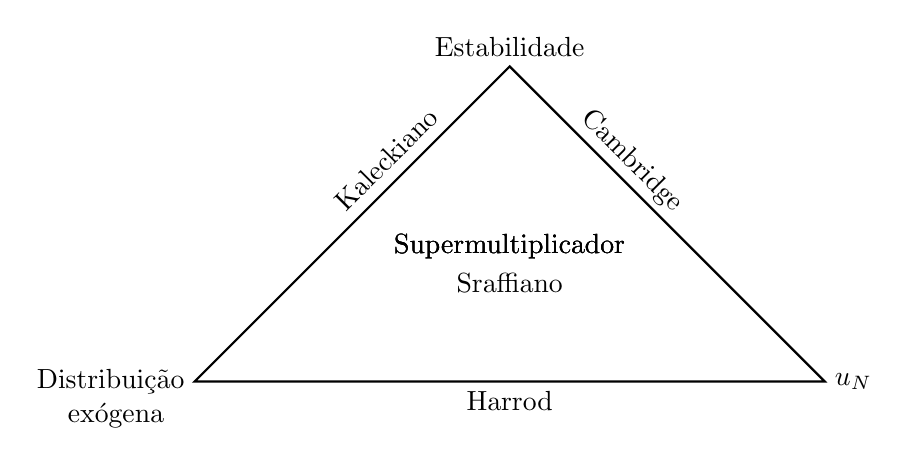
\begin{tikzpicture}[thick]
			\path[draw] (-4,0)  coordinate [label= left:Distribuição] (A)
			
			-- ( 0,4)  coordinate [label=above:Estabilidade] (C)
			-- ( 4,0)  coordinate [label=right:$u_N$] (B)
			-- cycle;
			\foreach \point in {A,B,C}
			\draw
			-- (0,2) node[anchor=north]{Supermultiplicador};
			\draw
			-- (-5,-0.15) node[anchor=north]{exógena};
			\draw
			-- (0,1.5) node[anchor=north]{Sraffiano};
			\draw
			-- (-1.75,3) node[anchor=north, rotate=45]{Kaleckiano};
			\draw
			-- (1.75,3) node[anchor=north, rotate=-45]{Cambridge};
			\draw
			-- (0,0) node[anchor=north]{Harrod};
			\end{tikzpicture}
		}
	\end{center}
	\caption*{\textbf{Fonte:} Elaboração própria}
\end{figure}
No entanto, da revisão da literatura verifica-se que tal mérito não se restringe ao SSM uma vez que uma vertente kaleckiana tem incluído gastos autônomos não criadores de capacidade produtiva por meio do princípio do ajuste do estoque de capital no \textbf{longo prazo}.
Sendo assim, é possível avançar em direção a um mapeamento de uma possível convergência entre os modelos sraffianos do tipo supermultiplicador e os modelos kaleckianos e então selecionar o caminho a ser seguido.
Antes de prosseguir, no entanto, cabe destacar que por serem modelos na fronteira da literatura, podem não ser representativos do que se entende por modelo kaleckiano e, por conta disso, serão denominados ``não-convencionais'' ao longo desta seção.

Em linhas gerais, tais modificações nos modelos kaleckianos estão associadas a algumas críticas envolvendo tanto a não convergência ao grau de utilização normal no longo prazo quanto a instabilidade decorrente da endogeinização do componente autônomo do investimento \cites{dallery_kaleckian_2007}{skott_theoretical_2012}{hein_harrodian_2012}.
A partir da contribuição de \textcite{allain_tackling_2015}, as alterações no modelo canônico têm a inclusão de gastos autônomos como denominador comum.
Uma vez introduzidos estes gastos, a poupança agregada --- assim como no SSM de \textcite{serrano_sraffian_1995} --- torna-se
$$
\frac{S}{Y} = s - \frac{Z}{Y}
$$
Neste ponto, \textcite[p.~10]{allain_tackling_2015} segue \textcite{serrano_sraffian_1995} em que a presença dos gastos autônomos possibilita o ajuste da identidade entre investimento e poupança pela participação desses gastos na renda e não por mudanças no grau de utilização. 

Dito isso, o autor prossegue para o médio prazo\footnote{
	Uma das distinções \textcite{allain_tackling_2015} são as caracterizações do curto, médio e longo prazo. O primeiro é definido pela não alteração dos gastos autônomos enquanto o segundo pode ser definido como aquele que tais gastos crescem a taxa exogenamente determinada. Por fim, o longo prazo é caracterizado por uma função de investimento harrodiana com o grau de utilização convergindo ao desejado. Vale pontuar a distinção com a temporalidade encontrada em \textcite{freitas_growth_2015} em que a convergência ao grau de utilização normal se dá na \textit{fully-adjusted position} enquanto a convergência da taxa de crescimento a $g_Z$ é dada no longo período. Para manter a comparatividade entre os modelos kalekicanos não-convencionais, adota-se a caracterização de \textcite{allain_tackling_2015} ao longo desta seção.
} em que a participação dos gastos autônomos na renda ($z$)\footnote{A rigor, o autor define essa participação dos gastos autônomos normalizados pelo estoque de capital e não pela renda, mas tal apresentação não altera a exposição ao longo do texto.} varia de acordo com a diferença entre as taxas de crescimento dos gastos autônomos e a efetiva ($g$):
\begin{equation}
\Delta z = (g_Z - g)\cdot z_{t-1}
\end{equation}
No curto ($g_Z = 0$) e médio prazo ($u \neq u_N$), o investimento das firmas não é totalmente induzido ($\gamma \neq 0$) de modo que sua taxa de crescimento é dada por
$$
g_I = \gamma + \gamma_u\cdot (u - u_n)
$$
em que $\gamma$ é expectativa tendencial de crescimento.
Quando a taxa de crescimento efetiva da economia se difere da taxa de crescimento dos gastos autônomos ($g\neq g_Z$),  haverá uma variação na participação dos gastos autônomos ($\Delta z$), impactando a demanda agregada e a taxa de poupança. 
Sendo assim, no médio prazo, a taxa de crescimento da economia converge a taxa dos gastos autônomos por meio de alterações da participação dos gastos autônomos na renda de modo que o grau de utilização é dado por:

\begin{equation}
\label{u_Allain}
u = \frac{g_z - \gamma}{\gamma_u} + u_N
\end{equation}
Esta equação evidencia que se, e somente se, a expectativa tendencial de crescimento ($\gamma$) for igual à taxa de crescimento dos gastos autônomos, o grau de utilização será igual ao normal no médio prazo e, portanto, é meramente acidental. No entanto, a convergência do grau de utilização ao normal é uma característica do longo prazo que decorre do princípio de ajuste do estoque de capital em que a taxa de crescimento esperada se adequa aos distanciamentos entre o grau de utilização efetivo e normal como pode ser visto na equação \ref{eqAllain}.
Além disso, \textcite{allain_tackling_2015} também destaca que para não incorrer na instabilidade no modelo kaleckiano canônico é necessário que o investimento deixe de ser autônomo: 
\begin{equation}
\label{eqAllain}
\Delta \gamma = \phi\gamma_u(u - u_N)
\end{equation}
em que $\phi$ é um fator de ajuste positivo e suficientemente pequeno\footnote{
	Além disso, \textcite[p.~14]{allain_tackling_2015} argumenta que a novidade  é o parâmetro  de ajustamento positivo ($\phi > 0$) que além de não implicar instabilidade Harrodiana, é também condição de estabilidade do modelo.
}.
Dito isso e partindo do equilíbrio de médio prazo e supondo um aumento na taxa de crescimento dos gastos autônomos, obtém-se um cenário em que a taxa efetiva de crescimento aumenta. 
Inicialmente, tanto a participação dos gastos autônomos na renda quanto o grau de utilização aumentam enquanto a taxa de investimento diminui.

No longo prazo, instaura-se o princípio do ajuste do estoque de capital e, como consequência disso, as firmas alteram a taxa de crescimento do investimento ajustar o estoque de capital e, assim, a participação dos gastos autônomos na renda diminui.
Em outras palavras, a medida que $\gamma$ aumenta, o grau de utilização vai convergindo ao normal enquanto a taxa dos gastos autônomos reduz.
Este processo de ajustamento de $\gamma$ se esgota com a convergência do grau de utilização ao normal de modo que 
taxa de crescimento efetiva se ajusta à taxa de crescimento dos gastos autônomos ($g = g_z$): 
%Em linha com \textcite{fagundes_role_2017}, argumenta-se que no \textbf{longo prazo} os modelos kaleckianos não-convencionais respondem suficientemente bem à convergência do grau de utilização sem incorrer na instabilidade
$$
\gamma = g = g_Z \Leftrightarrow u \to u_N
$$
Dito isso, cabe destacar os resultados de longo prazo:
(i) Mudanças na distribuição de renda geram alterações no nível, mas não na taxa final de crescimento, eliminado o paradoxo dos custos; 
(ii) o mesmo vale para alterações na propensão marginal a poupar e o paradoxo da parcimônia; 
(iii) o grau de utilização converge ao normal e 
(iv) aumento da taxa de crescimento dos gastos autônomos tem impactos positivos sobre a taxa de acumulação.
%Além disso, vale destacar que tal convergência decorre de uma das soluções do modelo é a equivalência entre o componente autônomo do investimento e a taxa de crescimento dos gastos autônomos. 
Como consequência indireta da crítica do supermultiplicador sraffiano, não raro encontram-se modelos kaleckianos (não-convencionais) com convergência ao grau de utilização normal que destacam a manutenção dos resultados kaleckianos canônicos na média:
	
	\begin{citacao}
		\textit{Thus, \textbf{on average}, the rate of utilization and the growth rate of the economy are higher than at the starting and terminal points of the traverse. Thus, what these Sraffians are telling us is that more attention should be paid to the average values
		achieved during the traverse than to the terminal points.} \cite[p.~408, grifos adicionados]{lavoie_post-keynesian_2015}
	\end{citacao}	

%%%%%%%%%%%%%%%%%%%%%%%%%%%%%%% Início Fagundes e Freitas %%%%%%%%%%%%
Para encerrar essa discussão, é feita uma comparação entre as dois fechamentos restantes, qual sejam, kaleckiano não-convencional e sraffiano.  Diante disso, existem duas questões importantes em aberto: (i) dadas as hipóteses compartilhadas, qual a distinção fundamental entre ambos os modelos? (ii) dados os objetivos desta investigação, qual modelo a ser adotado? 

O primeiro ponto pode ser respondido de forma mais direta: a principal diferença é a autonomia do investimento no médio prazo.  Resumidamente, se o investimento produtivo for induzido, a convergência ao grau de utilização normal é uma derivação do princípio do ajuste do estoque de capital e, dados certos limites, a capacidade produtiva se ajusta à demanda efetiva:

\begin{citacao}
	\textit{Indeed, the true reason for the lack of balance between capacity and demand in the Oxford theory [Modelos kaleckianos] in the long run is actually much simpler. As we have seen above in this theory, in the long run the level of output adapts itself to the level of aggregate demand. The level of productive capacity, however, cannot adjust to this level of aggregate demand because current capacity has already been determined as the result of previous autonomous investment. Hence it is the idea that investment is \textbf{autonomous} and not \textbf{anything related to oligopoly} or competition that explain the long-run discrepancies between capacity and demand.}
	\cite[p.~120, grifos adicionados]{serrano_sraffian_1995}
\end{citacao}
Por outro lado, se o investimento possuir um componente autônomo, como nos modelos kaleckianos convencionais, a capacidade produtiva também se torna autônoma de modo que o ajuste entre demanda e oferta recai sobre o grau de utilização:
\begin{citacao}
	\textit{Note that from our definition of capacity generating investment expenditures, it follows that when this type of investment is induced, productive capacity is necessarily a consequence of the evolution of effective demand. On the other hand, when capacity generating investment is autonomous it is productive capacity that emerges as a necessary consequence of (autonomous) investment. […] Indeed, the view that capacity of each sector is adjusted to normal level of effectual demand in every long-period position, necessary implies treating the long-period level of capacity generating investment as an endogenous magnitude.} \cite[p.~77]{serrano_sraffian_1995}
\end{citacao}
Como mostrado ao longo desta seção, isso deixa de ser o caso nos modelos kaleckianos com investimento induzido no longo prazo.

Para responder a segunda questão, resta esclarecer um possível ponto de estranhamento. O principal objetivo desta pesquisa é investigar os determinantes do ciclo econômico norte-americano e desenvolver um modelo que ajude a esclarecer alguns dos fatos estilizados da economia norte-americana dos anos 1992 a 2019. Sendo este o caso, a ênfase na discussão de modelos de longo prazo parece ser desconexa. 
No entanto, como mencionado na introdução, os modelos elegíveis são aqueles aderentes a alguns fatos estilizados (\textit{e.g.} relação positiva entre taxa de investimento e crescimento)  no curto, médio e longo prazo.
Desse modo, optar por modelos que se mostram adequados para o curto- e longo-prazo, mas não para o médio-prazo se mostra questionável uma vez que a validade dos resultados está restrita a uma certa temporalidade. 

%TODO Rever temporalidade
Os modelos discutidos nessa seção --- vale lembrar, kaleckiano não-convencional e supermultiplicador sraffiano --- representam alguns fatos estilizados no curto prazo e na posição plenamente ajustada (equivalente ao longo prazo kaleckiano). Resta verificar se o mesmo vale enquanto a propensão marginal a poupar não está ajustada (denominado aqui por  \textbf{médio prazo})\footnote{Esta parte da exposição é inspirada na contribuição de \textcite{fagundes_role_2017} no que diz respeito ao médio prazo.}. 
%TODO Rever se o tratamento de médio prazo está adequado
%Dito isso, dentre os modelos kaleckianos com gasto autônomo e principio de ajuste do estoque de capital e supermultiplicador sraffiano, resta selecionar aquele reproduza o fato estilizado da relação positiva entre taxa de investimento e taxa de crescimento. 
Dito isso, seja $i$ a taxa de investimento, $\gamma_A$ a parcela autônoma e $h$ a parcela induzida do investimento (das firmas) de modo que a representar a função de acumulação kaleckiana pode ser reescrita como\footnote{
	As etapas são:
	$$
	\frac{I}{K}  = \gamma + \gamma_uu - \gamma_uu_N
	$$
	
	$$
	\gamma_A = \gamma - \gamma_uu_N
	$$
	
	$$
	I = (\gamma_A + \gamma_uu)K
	$$
	
	$$
	\gamma_u\cdot u \cdot K \equiv \gamma_u\frac{Y}{Y_{FC}}K \equiv \gamma_u\cdot v\cdot Y
	$$
	
	$$
	I = \gamma_A\cdot K + \gamma_u\cdot v\cdot Y
	$$
}

\begin{equation}
\tag{kaleckiana}
I = \gamma_A\cdot K + h\cdot Y
\end{equation}
enquanto a do supermultiplicador (adiante, SSM) continua sendo

\begin{equation}
\tag{SSM}
I = h\cdot Y
\end{equation}
Como destacado na seção \ref{SecHarrod}, na ausência de gastos autônomos, a propensão marginal e média a poupar são iguais e, portanto, no modelo kaleckiano convencional, a taxa de investimento é determinada pela taxa de poupança definida exogenamente. Incluindo os gastos autônomos neste modelo, obtém-se:

$$
i = \frac{i_{Trad}\gamma_A + hz}{\gamma_A + z}
$$
em que $i_{Trad}$ denota, tal como em \textcite{fagundes_role_2017}, a taxa de investimento no modelo kaleckiano canônico. Nos modelos kaleckianos não-convencionais, a ausência dos gastos autônomos implica a volta ao modelo kaleckiano convencional enquanto no supermultiplicador retorna-se ao \textcite{harrod_essay_1939}. Mais uma vez, a introdução de tais gastos não é capaz, por si só, de eliminar a instabilidade, mas sim pela modificação da função investimento \textit{à la} acelerador flexível cuja alteração é feita somente no longo prazo nos modelos derivados de \textcite{allain_tackling_2015}. 

Prosseguindo com a exposição e analisando o equilíbrio de \textit{steady growth} com gastos autônomos ($Z > 0$), verifica-se que no médio prazo dos modelos kaleckianos não-convencionais ($g\to g_Z$), a taxa de investimento ($i_{MR}$) é dada por:
\begin{equation}
\label{investoFagundes}
i_{MR} = \frac{h\cdot g_Z}{g_Z - \gamma_A}
\end{equation}
Diante deste resultado, \textcite{fagundes_role_2017} argumentam que a inclusão dos gastos autônomos no modelo não garante a convergência do grau de utilização ao normal. Para que tal tendência ocorra, por sua vez, é necessário que a participação da parcela autônoma do investimento convirja a zero ($\gamma_A \to 0$) e isto ocorre, por exemplo, no modelo de  \textcite{lavoie_convergence_2016}. 
No entanto, \textcite{fagundes_role_2017} reportam que de acordo com este modelo, uma economia que cresce a taxas maiores é aquela que apresenta uma menor taxa de investimento que, por sua vez, contradiz a evidência econométrica a respeito do fato estilizado da relação \textbf{positiva} entre taxa de crescimento e  taxa de investimento \cites{braga_investment_2018}{haluska_growth_2019}. Supondo, por simplificação, que as variações são infinitesimais, isto pode ser explicitado em termos da equação \ref{investoFagundes} por derivadas parciais:
$$
\frac{\partial i_{MR}}{\partial g_Z} = - \frac{\gamma_A h}{[g_Z - \gamma_A]^2} < 0 \Leftrightarrow \gamma_A > 0
$$
Além disso, os autores pontuam um problema de ``dupla identidade'' nos modelos \textit{à la} \textcite{allain_tackling_2015} decorrente das diferentes condições de equilíbrio, um com e outro sem gastos autônomos, cujos padrões de crescimento são mutualmente excludentes. No primeiro, obtém-se um regime liderado pelo investimento produtivo, mas incapaz de gerar a tendência do grau de utilização ao normal e de destacar a importância dos gastos autônomos ($Z\to 0$). No outro, ocorre o inverso, um regime liderado pelos gastos autônomos ($\gamma_A \to 0$), mas apresenta uma relação negativa entre crescimento e taxa de investimento. Ambos os casos contrariam
o fato estilizado da convergência do grau de utilização da capacidade produtiva ao normal \cite{gahn_empirical_2019} quanto a relação positiva entre crescimento e taxa de investimento \cites{braga_investment_2018}{haluska_growth_2019}. Portanto, a aceitação a conclusão de \textcite[p.~13]{fagundes_role_2017} é imediata:

\begin{citacao}
	
	[I]\textit{f we think of such a model as an intermediate step towards the long-run model, then we
	believe that there is no problem in using it. The problem occurs when we think of the medium-run
	model as a contribution to the understanding of economic reality in itself, independent from the long-run model}.
\end{citacao}
Neste ponto, o trecho a seguir é esclarecedor:

\begin{citacao}
	\textit{What the supermultiplier adds to the neo-Kaleckian framework is a plausible mechanism for explaining phases
	of the business cycle when the output share of capacity investment is rising amidst robust rates of output growth.} \cite[p.~9]{fiebiger_trend_2017}
\end{citacao}

Resta checar se a alternativa pelo SSM incorre nos mesmos problemas. Para isso, basta verificar os resultados para o caso em que o investimento é completamente induzido. Como a alternativa kaleckiana com gastos autônomos pode ser considerada como híbrida entre o modelo kaleckiano convencional e o SSM, basta substituir $\gamma_A = 0$ na equação \ref{investoFagundes}, obtendo:
$$
i_{MR} = \frac{I}{Y} =  h
$$
Seguindo a proposta do supermultiplicador em que o investimento é completamente induzido:
$$
g = \frac{h\cdot u}{v} \Rightarrow h = i_{MR} = \frac{g_Z\cdot v}{u}
$$

$$
\frac{\partial i_{MR}}{\partial g_Z} = \frac{v}{u} > 0
$$
Portanto, a relação negativa entre crescimento e taxa de investimento deixa de existir e isso não é feito à custa da não convergência do grau de utilização ou da relevância dos gastos autônomos no longo prazo. 
Diante desta discussão, conclui-se que o modelo do SSM não é incompatível para analisar o médio prazo ou restrito ao longo prazo como afirma \textcite{nikiforos_comments_2018}. Com isso, chega-se a conclusão de que o supermultiplicador sraffiano como o mais adequado para atender os objetivos desta pesquisa. 


%TODO TRANSIÇÃO SEÇÃO SEGUINTE




\section{Gastos autônomos nos modelos de crescimento}\label{SecAutonomos}

\subsection{Um breve mapeamento da fronteira heterodoxa}
\label{Hibridos}


Ao longo desta seção, serão mapeados os modelos de crescimento, 
sejam eles kaleckianos ou sraffianos, liderados pelos gastos autônomos não criadores de capacidade produtiva ao setor privado ($Z$). Isso não implica que são os únicos modelos com gastos autônomos, mas sim, que são os modelos em que a dinâmica destes gastos não é esgotada no longo prazo\footnote{
	No que diz respeito ao consumo financiado por crédito, por exemplo, destacam-se os trabalhos de \textcite{dutt_maturity_2006}, \textcite{palley_inside_2010} e \textcite{hein_finance-dominated_2012}.
	No entanto, esses autores trabalham no arcabouço kaleckiano básico. Por isso, a estabilidade só é garantida se o consumo financiado por crédito a crescer a mesma taxa que a acumulação --- ou seja, este componente do consumo não pode ser tratado como de fato um gasto autônomo.
	Diante desta limitação, \textcite{pariboni_household_2016} argumenta que os gastos autônomos desempenham um papel passivo e sugere uma alternativa a partir do supermultiplicador sraffiano. Desta forma, a causalidade anterior é revertida de modo que a taxa de acumulação convirja gradualmente a taxa de crescimento consumo financiado por crédito.
}.
Para manter a comparatividade entre os modelos apresentados, serão realçados alguns dos resultados de \textbf{longo prazo}, são eles: (i) mudanças na distribuição de renda; (ii) alterações na propensão marginal propensão a poupar; (ii) convergência do grau de utilização ao normal; (iv) aumento da taxa de crescimento dos gastos autônomos. Por fim, as variáveis serão adaptadas de modo que $\gamma$ é o componente autônomo do investimento,  $z$ é a participação dos gastos autônomos ($Z$) na renda que crescem a taxa $g_Z$.
Feitas essas ressalvas e seguindo a tipologia de \textcite{cesaratto_technical_2003} e a categorização de \textcite{serrano_sraffian_1995}, tais gastos autônomos são: (i) gastos do governo; (ii) consumo financiado por crédito; (iii) Investimento residencial; (iv) Gastos com P\&D\footnote{
	%TODO Nota sobre especificidade do investimento em P\&D.
	Por mais que os gastos com P\&D são contabilmente considerados investimento das firmas, optou-se por incluí-los para avaliar modelos que partem do supermultiplicador sraffiano e consideram tais gastos como sendo os determinantes da dinâmica.
} e; (v) Exportações.


%% Modelo Allain
%TODO Comparar com a versão do artigo dele
No já mencionado modelo de \textcite{allain_tackling_2015}, os gastos do governo além de serem autônomos não criam capacidade ($Z$) e são financiados por impostos que se ajustam endogenamente para manter o saldo primário equilibrado\footnote{
	Dentre os resultados particulares do modelo de \textcite{allain_tackling_2015}, pontua-se os efeitos contra-cíclicos do gasto público sobre o nível de atividade e seu papel enquanto estabilizador automático do crescimento.
}.  
Os resultados de longo prazo são:
	(i) Mudanças na distribuição de renda geram alterações no nível, mas não na taxa de crescimento, eliminado o paradoxo dos custos; 
	(ii) o mesmo vale para alterações na propensão marginal a poupar e o paradoxo da parcimônia; 
	(iii) o grau de utilização converge ao normal e 
	(iv) aumento da taxa de crescimento dos gastos autônomos tem impactos positivos sobre a taxa de acumulação\footnote{
		A convergência do grau de utilização ao nível normal implica na eliminação dos paradoxos kaleckianos em termos de taxas. Além disso, vale destacar que tal convergência decorre de uma das soluções do modelo é a equivalência entre o componente autônomo do investimento e a taxa de crescimento dos gastos autônomos. Como consequência indireta da crítica do supermultiplicador sraffiano, não raro encontram-se modelos kaleckianos (não-convencionais) com convergência ao grau de utilização normal que destacam a manutenção dos resultados canônicos na média:
	
		\begin{citacao}
			Thus, \textbf{on average}, the rate of utilization and the growth rate of the economy are higher than at the starting and terminal points of the traverse. Thus, what these Sraffians are telling us is that more attention should be paid to the average values
			achieved during the traverse than to the terminal points. \cite[p.~408, grifos adicionados]{lavoie_post-keynesian_2015}
	\end{citacao}
	
}.


%MODELO HEIN (2018): GASTOS DO GOVERNO E SUSTENTABILIDADE DA DÍVIDA
Por mais que o modelo de \textcite{allain_tackling_2015} inclua os gastos do governo como sendo os gastos autônomos e preserve as características dos modelos kaleckianos (em nível), \textcite{hein_autonomous_2018} argumenta que não inclui uma discussão sobre a dinâmica do \textit{déficit} e da dívida pública no longo prazo. 
Dito isso, insere as modificações de \textcite{allain_tackling_2015} no arcabouço contábil da metodologia \textit{Stock-Flow Consistent} (adiante, SFC) de modo que os gastos do governo passam a ser financiados por crédito e emissão monetária\footnote{
	Como consequência, \textcite{hein_autonomous_2018} afirma que este modelo permite incluir o paradoxo da dívida, ou seja, redução da dívida pública como resultado de um aumento dos gastos do governo dado o aumento do consumo a partir da riqueza financeira. 
}. Uma distinção deste modelo é que o autor julga não ser razoável, dada a incerteza keynesiana fundamental, que o grau de utilização convirja ao normal no longo prazo\footnote{
	Dentre as equações para o equilíbrio de longo prazo, cabe mencionar àquela que diz respeito ao grau de utilização. Adaptando as variáveis,
	$$
	u = \frac{g_z - \gamma}{\gamma_u}
	$$
	que indica que o grau de utilização não converge ao nível normal e pode se manter persistentemente em um patamar elevado a depender dos parâmetros. Além disso, se os gastos autônomos crescerem a uma mesma taxa que o valor do \textit{animal spirits}, o grau de utilização será nulo. Em outras palavras, como a estabilidade independe de ($\gamma$), não existem restrições para esse parâmetro de modo que possa zerar o grau de utilização. Dito isso, conclui-se que tal equação deve estar incompleta e deveria ser
	$$
	u = \frac{g_z - \gamma}{\gamma_u} + u_n
	$$
}. 
Dito isso, cabe realçar os resultados que tocam os objetivos desta seção\footnote{
	Dentre os resultados restritos a esse modelo, destaca-se:  
	(a) Mudanças nos \textit{animal spirits} afetam negativamente o grau de utilização, mas não possuem efeitos na taxa de crescimento; 
	(b) redução do \textit{déficit} e da dívida do governo em decorrência de: 
	(b.i) aumento nos \textit{animal spirits}; 
	(b.ii) diminuição da propensão marginal a poupar e aumento da propensão a consumir a partir da riqueza. 
	Além disso, o autor conclui, tal como \textcite[Capítulo 11]{godley_growth_2011} e \textcite{arestis_effectiveness_2012}, que uma política fiscal ativa pode atuar para aquecer a economia sem implicar em insustentabilidade da dívida pública.
}: 
	(i) Mudanças na distribuição de renda não afetam a taxa de crescimento de longo prazo; 
	(ii) o mesmo vale para mudanças na propensão marginal a poupar e a consumir a partir da riqueza; 
	(iii) Aumento na taxa de crescimento dos gasto do governo ($g_Z$) afetam positivamente o grau de utilização que, por sua vez, não converge ao normal\footnote{
		Vale mencionar que uma das peculiaridades deste modelo é a endogeinização da distribuição funcional da renda pelo grau de utilização. No entanto, tal resultado pode decorrer da diferenciação feita por \textcite{hein_autonomous_2018} entre renda decorrente da produção e renda financeira.
		}; 
	(iv) A taxa de crescimento da economia converge para a taxa de crescimento dos gastos autônomos no longo prazo. 

%MODELO BROCHIER (2018): RIQUEZA FINANCEIRA ACUMULADA
Outro modelo SFC com gasto do governo é o de \textcite{brochier_supermultiplier_2018}.
A principal diferença em relação é a endogeinização dos gastos autônomos por meio do consumo a partir da riqueza financeira acumulada\footnote{
	Outro modelo com consumo a ser destacado é o de \textcite{nah_role_2019} %NAH E LAVOIE (2019): INFLAÇÃO E DISTRIBUIÇÃO ENDÓGENA
	que inclui inflação por conflito distributivo. Por mais que tal modelo apresente gastos autônomos como os demais nesta seção, a endogeinização da distribuição de renda elimina uma das hipóteses compartilhadas entre os modelos analisados e, portanto, compromente a comparação e deve ser discutido a parte.
}. 
Alguns dos resultados apresentados anteriormente se alteram: 
	(i) alterações na distribuição de renda impactam a taxa de acumulação no longo prazo; 
	(ii) aumento na propensão marginal a consumir a partir da renda disponível aumenta a taxa de crescimento de longo prazo; 
	(iii) grau de utilização converge ao normal; 
	(iv) aumento na propensão a consumir a partir da riqueza (componente correspondente ao $Z$) aumenta a taxa de acumulação. 
	Neste modelo, os paradoxos dos custos e da parcimônia são mantidos --- apesar dos mecanismos causais não estarem claros --- inclusive com o grau de utilização convergindo ao desejado, configurando uma possível exceção ao que foi exposto até então.

%TODO: Dúvida - Mencionar artigo sobre distribuição de renda.

%No entanto, a menção anterior ao governo não é ocasional. MIMEO argumentam que a presença do governo no modelo atua como a geração de um gasto autônomo que persiste enquanto efeito riqueza. Desse modo, a reformulação deste modelo para uma economia sem governo gera os resultados esperados tais como aqueles apresentados anteriormente: (i) mudanças na distribuição de renda não afetam a taxa de acumulação; (ii) o mesmo vale para a propensão marginal a poupar (via propensão marginal a consumir a partir dos salários); (iii) grau de utilização converge ao desejado; (iv) mudanças na propensão marginal a consumir a partir da riqueza acumulada não alteram a taxa de acumulação. Portanto, feitas essas modificações, os resultados apresentados anteriormente são restaurados e as exceções são eliminadas\footnote{Outra modificação verificada por MIMEO é o desenho da política fiscal e, tal como na retirado do governo, alteram os resultados obtidos na simulação.}.

%TODO: Evidenciar que os resultados diferentes da Lídia não estão no modelo do Mandarino


%TESE MANDARINO: CONSUMO FINANCIADO POR CRÉDITO
Outro modelo na linha do anterior --- mas sem retorno dos paradoxos kaleckianos --- é o de \textcite{mandarino_financing_2018} em que o consumo dos trabalhadores é financiado por crédito, adicionando um tratamento das relações financeiras ao modelo de \textcite{pariboni_household_2016} e de \textcite{fagundes_dinamica_2017}. No que diz respeito às implicações para o longo prazo, pontua-se\footnote{
	O modelo de \textcite{mandarino_financing_2018} apresenta diferentes cenários mas foram realçadas as conclusões que tangenciam os quatro pontos de comparação, qual sejam, mudanças: (i) na distribuição; (ii) na propensão marginal a poupar; (iii) do grau de utilização; (iv) decorrentes das variações de $g_Z$.
}: 
	(i) não foram simulados os efeitos de mudanças na distribuição de renda; 
	(ii) diminuição na propensão marginal média a poupar (via aumento na propensão marginal a consumir dos capitalistas) afeta negativamente o nível de atividade mas não a taxa de crescimento de longo prazo e; 
	(iii) grau de utilização converge ao desejado em todos os cenários; 
	(iv) aumento em $g_Z$ aumenta a taxa de acumulação de longo prazo.
Adicionalmente, este modelo é centrado nas condições de estabilidade do endividamento dos trabalhadores no longo prazo e conclui que aumentos da taxa de crescimento dos gastos autônomos bem como na taxa de juros implicam em diminuição da taxa de endividamento dos trabalhadores e das firmas. 


% MODELO NAH E LAVOIE (2019): CONSUMO AUTÔNOMO E INFLAÇÃO POR CONFLITO DISTRIBUTIVO E ENDOGEINIZAÇÃO DA DISTRIBUIÇÃO

%MODELO NAH AND LAVOIE: EXPORTAÇÃO
Analisados o consumo autônomo (financiado por crédito e riqueza) e os gastos do governo, restam os demais componentes da demanda agregada.
No modelo de \textcite{nah_long-run_2017}, semelhante ao de \textcite{dejuan_hidden_2017}, as exportações desempenham o papel dos gastos autônomos. Mais especificamente, é uma proposta para estender a contribuição de \textcite{serrano_sraffian_1995} para o caso de uma economia aberta suficientemente pequena. Os resultados de longo prazo são iguais aos apresentados anteriormente e por conta disso não serão repetidos. No entanto, este modelo se destaca pelo regime de acumulação pode ser caracterizado como \textit{wage-} ou \textit{profit-led} a depender da sensibilidade da taxa de câmbio real a mudanças na distribuição de renda. 

%MODELO DUTT: INOVAÇÃO
Por mais que estes modelos consigam dar atenção para diferentes gastos autônomos, \textcite{dutt_observations_2018} afirma que são incapazes de fazer com que o investimento (criador de capacidade produtiva) seja determinante do crescimento no longo prazo tal como em Kalecki. Para tanto, inclui um componente de crescimento que expressa o progresso tecnológico determinado autonomamente. No entanto, tal formulação não faz com que o grau de utilização convirja ao normal e que a taxa de crescimento seja determinada pelos gastos autônomos uma vez que essa nova variável afeta a capacidade produtiva no longo prazo. Para garantir as propriedades do supermultiplicador, o progresso técnico é endogeneizado pelos gastos com P\&D ($g_R$) de forma que:
$$
g_I + g_R = g_S
$$
Neste modelo, uma vez cessados os efeitos do progresso tecnológico: 
	(i) distribuição afeta a taxa de crescimento de médio prazo apenas; 
	(ii) propensão marginal a poupar também não afeta o crescimento, mas determina a condição de estabilidade; 
	(iii) grau de utilização converge ao normal; 
	(iv) taxa de crescimento converge para a taxa de crescimento dos gastos com P\&D e o resultado se preserva com mais de um gasto autônomo. 
Portanto, partindo desta formulação, o progresso tecnológico pode determinar o ritmo de crescimento no longo prazo sem afetar o investimento.

Apesar dessa variabilidade de modelos, destaca-se a escassez daqueles que tratam do investimento residencial em específico. 
Sendo assim, cabe a seção seguinte avaliar como incluí-lo na agenda de pesquisa dos modelos de crescimento liderados pela demanda.

\section{Investimento residencial e crescimento: rumo a endogeinização}
\label{RevResidencial}

INTRODUÇÃO

INDICAR QUE SERÁ FEITO UM ESFORÇO PARA TRATAR DO INVESTIMENTO RESIDENCIAL DE FORMA TEÓRICA APESAR DE COMUMENTE ASSOCIADO A EMPIRIA.


INVESTIMENTO RESIDENCIAL E DESENVOLVIMENTO

Por se tratar de um gasto não criador de capacidade produtiva, o debate\footnote{Para mais detalhes, ver \textcite{arku_housing_2006}.} se restringiu em categorizá-lo enquanto absorvedor de recursos produtivos \cite{solow_importance_1995} enquanto parte da literatura de crescimento indicava  a possibilidade de um sobreinvestimento residencial \cite{mills_has_1987}.

TEXTO NBER: PERDA DE IMPORTÂNCIA DESTE SETOR
ROGNLIE: REDUÇÃO DA TAXA DE CAPITAL

% Zezza
Examinada parcela dos trabalhos ortodoxos, cabe inspecionar a forma com que a heterodoxia tratou do tema. 
% Financeirização e hipotecarização
Parte significativa desta literatura  --- emergente no pós-crise imobiliária --- centra esforços na conexão deste tipo de gasto com processos mais gerais como a financeirização \cites{aalbers_financialization_2008}{bibow_financialization_2010} enquanto uma pequena fração aborda investimento residencial e crescimento.
A título de menção, vale destacar também o trabalho de \textcite{zezza_u.s._2008} em que são investigados os efeitos da diminuição da propensão marginal a poupar da economia norte-americana a partir da metodologia \textit{Stock-Flow Consistent} e conclui que o consumo financiado por crédito é o principal determinante do crescimento de modo que o investimento residencial um efeito riqueza via valorização dos imóveis apenas em que os ganhos de capital ajudam a explicar a redução na taxa de poupança apesar da distribuição da renda a favor dos lucros. 


ZEZZA, CARDACI, ETC: DISTRIBUIÇÃO E INVESTIMENTO RESIDENCIAL

HANSEN E DUESENBERRY: INVESTIMENTO RESIDENCIAL E DEMOGRAFICA

GOWANS E ALLAIN: INVESTIMENTO RESIDENCIAL E DEMOGRAFIA EM MODELOS DO TIPO SUPERMULTIPLICADOR

DESTA REVISÃO DA LITERATURA VERIFICA-SE QUE OS MODELOS OU RESTRINGEM A CONTRIBUIÇÃO DO INVESTIMENTO RESIDENCIAL A PERDA DA PARTICIPAÇÃO RELATIVA DOS SALÁRIOS OU CENTRAM A ANÁLISE EM ELEMENTOS DEMOGRÁFICOS ALÉM DE DEIXAR DE LADO A DEMANDA POR IMÓVEIS POR RAZÕES ESPECULATIVAS. COMO SERÁ MELHOR DISCUTIDO NO CAPÍTULO SEGUINTE, A RELEVÂNCIA DO INVESTIMENTO RESIDENCIAL NO EUA SE DÁ PELA CONEXÃO DESTE GASTO COM A AMPLIAÇÃO DO COLATERAL E SUBSEQUENTE ELEVAÇÃO DO ENDIVIDAMENTO/CONSUMO. UMA VEZ QUE ESTE CAPÍTULO É DE TEOR TEÓRICO, PRETENDE-SE DISCUTIR COMO INCLUIR TAL COMPONENTE DA DEMANDA AGREGADA SEM CONFINÁ-LO A UM CASO ESPECÍFICO.

- A AUTONOMIA DESTE GASTO NÃO SE RESTRINGE AO CRESCIMENTO POPULACIONAL.
- INCLUSÃO DE ELEMENTOS DA OFERTA DE TRABALHO NÃO PODEM SER DESASSOCIADOS DE UMA DISCUSSÃO SOBRE TÉCNICAS PRODUTIVAS DE MODO QUE OUTRAS QUESTÕES SURGEM

NIKALDI

TAXA PRÓPRIA DE JUROS

Como destaca \textcite[p.~53]{teixeira_crescimento_2015}, os detentores de um ativo levam seu preço em consideração no processo decisório uma vez que sua variação pode gerar perdas/ganhos de capital. Como alternativa, elabora a taxa própria de juros do imóveis (Taxa Própria, $own$) definida como a taxa de juros hipotecária ($r_{mo}$) deflacionada pela inflação dos imóveis ({$\dot p_h$}) de modo que o investimento residencial ($g_Z$) é dado por:
$$
g_Z = \phi_0 - \phi_1 \overbrace{\left(\frac{1+r_{mo}}{1+\dot p_h} - 1\right)}^{\text{Taxa Própria}}
$$

\begin{equation}
g_Z = \phi_0 - \phi_1\cdot own
\end{equation}
em que os $\phi_i$s são parâmetros e cujo termo em parênteses é a Taxa Própria. 
O primeiro parâmetro se refere aos determinantes de longo prazo (\textit{e.g.} arranjos institucionais do mercado imobiliários e de crédito) enquanto o segundo capta a demanda por imóveis decorrente das expectativas de ganhos de capital resultantes da especulação com o estoque de imóveis existente e diz respeito ao ciclo econômico.

Em outras palavras, a taxa de juros das hipotecas capta o serviço da dívida para os ``investidores'' (neste caso, famílias) enquanto a variação do preço dos imóveis permite incorporar mudança no patrimonio líquido. Portanto, aufere de modo satisfatório o custo real em imóveis de se comprar imóveis \cite[p.~53]{teixeira_crescimento_2015}. Desse modo, a partir da taxa própria de juros do imóveis é possível revelar importância do investimento residencial para além do ciclo e estendê-la para o longo prazo.  Tal proposta, portanto, lança luz sobre a influência da inflação imobiliária na construção de novos imóveis e, de acordo com o supermultiplicador sraffiano, sobre o produto como um todo. 


%

\section{Gastos autônomos não criadores de capacidade e a instabilidade velada}\label{Literatura}

A presente seção tem por objetivo destacar como os modelos Kaleckianos incorporaram os gastos autônomos não criadores de capacidade produtiva ao setor privado ($Z$). Antes de prosseguir, no entanto, cabe destacar que por serem modelos na fronteira da literatura, podem não ser representativos do que se entende por modelo Kaleckiano. Desse modo, ao longo desta seção, estão sendo analisados modelos kaleckianos não-tradicionais\footnote{Manifestação deste não-consenso é a divergência do significado econômico do componente autônomo do investimento.}. Além disso, a inclusão deste componente de gasto revela a resolução parcial da instabilidade harrodiana nos modelos Kaleckianos\footnote{Como visto, nos modelos mais convencionais, portanto, a endogeneidade do grau de utilização é suficiente para contornar esse problema. As complicações mencionadas, decorrem das sofisticações dos modelos Kaleckianos.}. A razão do porquê pode ser explicitada seguindo a exposição de \textcite{hein_harrodian_2012}\footnote{Apresentação semelhante pode ser encontrada em \textcite{allain_macroeconomic_2014}}. 

%INICIO EXPOSIÇÃO
Considerando, como em \textcite{amadeo_role_1986}, que o investimento reaja às expectativas sobre o grau de utilização ($u^e$), a função de acumulação ($g_I$) pode ser reescrita como:

\begin{equation}
\label{Kalecki_Autonomous}
g_I = \gamma + \gamma_u (u^e - u_n)
\end{equation}
em que $\gamma$ corresponde ao componente autônomo do investimento e pode ser traduzido tanto como \textit{animal spirits} quanto expectativa média da taxa de crescimento de longo prazo \cite[p.~4]{allain_macroeconomic_2014}.
No curto prazo, o grau de utilização da capacidade pode ser diferente do grau de utilização de equilíbrio. Se as firmas ajustam o estoque de capital para que o grau de utilização esteja no nível desejado, tais expectativas devem ser revistas:

\begin{equation}
\Delta u^e = \xi (u - u^e), \hspace{3cm} \xi > 0
\end{equation}
Da mesma forma, as expectativas em relação à taxa de crescimento secular ($\gamma$) são corrigidas pelas taxas de crescimento efetivas ($g^*$), ou seja, 
\begin{equation}
    \Delta \gamma = \phi (g^* - \gamma)
\end{equation}
em que $\phi$ indica um fator de correção positivo. Substituindo recursivamente, obtém-se:
\begin{equation}
    \Delta \gamma = \phi \gamma_u (u - u^e) \Leftrightarrow \Delta g_I = \varphi (u^e - u_n), \hspace{2cm} \varphi > 0
\end{equation}

Tal equação implica na instabilidade de Harrod uma vez que há uma sobre/sub-estimação do grau de utilização de equilíbrio que, por sua vez, se afasta cada vez mais do grau de equilíbrio. Essa instabilidade\footnote{Vale destacar que não é necessário recorrer à mudanças nos modelos Kaleckianos para incorrer em instabilidade, como pontua \textcite{dallery_kaleckian_2007}, o que não implica que todas elas são do tipo Harrodiana.}, argumentam \textcite{hein_harrodian_2012}, decorre do coeficiente $\gamma$ da função de investimento que deixa de ser constante na medida que o grau de utilização se afasta do normal. Nesses termos, não é paradoxal um modelo apresentar estabilidade Keynesiana e não resolver a instabilidade Harrodiana\footnote{Para mostrar que este problema não se restringe a uma parcela desses modelos, é apresentado mesmo raciocínio para a equação de acumulação que inclui a sensibilidade do investimento à participação dos lucros na renda nos moldes de \textcite{bhaduri_unemployment_1990}:

\begin{equation}
\label{KaleckiHarrod}
\begin{split}
    \dot \gamma = &\xi (g^* -\gamma), \hspace{3cm} \xi > 0\\
     = &\xi[\gamma_u (u-u_n) + \gamma_\pi\pi]
\end{split}
\end{equation}
A equação acima indica que $\dot \gamma$ é necessariamente positivo, o que faz com que a taxa de crescimento se afaste da taxa de longo prazo. Em outras palavras, a instabilidade harrodiana está presente nos modelos Kaleckianos tradicionais com correção das expectativas no componente autônomo do investimento.}. 

Diante deste problema, foram feitas modificações nos modelos Kaleckianos convencionais para que a estabilidade Harrodiana fosse balizada. Grosso modo, tais mudanças têm a inclusão de gastos autônomos como denominador comum, mas uma mediação se faz necessária. Tal como aponta \textcite[p.~3]{allain_macroeconomic_2014}, os resultados são distintos a depender de quais gastos são considerados autônomos e isso será avaliado adiante. Para manter a comparatividade entre os modelos apresentados, serão realçados os resultados que dizem respeito a efeitos em comum no \textbf{longo prazo}\footnote{Destaca-se um ponto de concordância com \textcite{nikiforos_comments_2018} em que o supermultiplicador sraffiano é um modelo para longo prazo e deve ser avaliado enquanto tal. No entanto, isso não impede de incluir elementos cíclicos no modelo e será objeto do capítulo \ref{CapModelo}. Por enquanto, resta enfatizar a atenção dada aos resultados de longo prazo para torná-los devidamente comparáveis.}, são eles: (i) mudanças na distribuição de renda; (ii) alterações nas propensões à poupar; (ii) efeitos sobre o grau de utilização; (iv) impactos do aumento da taxa de crescimento dos gastos autônomos. Já aqueles resultados que são exclusivos do modelo analisado serão postos em evidência quando necessário.

%MODELO LAVOIE: EXPORTAÇÃO

%MODELO ALLAIN: GASTOS DO GOVERNO

%MODELO HEIN (2018): GASTOS DO GOVERNO E SUSTENTABILIDADE DA DÍVIDA

Por mais que o modelo de \textcite{allain_macroeconomic_2014} inclua os gastos do governo como sendo os gastos autônomos e preserve as características dos modelos Kaleckianos (em nível), \textcite{hein_autonomous_2018} argumenta que não inclui uma discussão sobre a dinâmica do \textit{déficit} e da dívida pública no longo prazo. Os gastos do governo, financiados por crédito e emissão monetária, crescem a uma taxa exógena tal como em \textcite{allain_macroeconomic_2014}. Uma distinção deste modelo é que o autor julga não ser razoável, dada a incerteza keynesiana fundamental, que o grau de utilização convirja ao normal no longo prazo\footnote{Dentre as equações para o equilíbrio de longo prazo, cabe mencionar àquela que diz respeito ao grau de utilização. Adaptando as variáveis,
$$
u = \frac{g_z - \gamma}{\gamma_u}
$$
que indica que o grau de utilização não converge ao nível normal e pode se manter persistentemente em um patamar elevado a depender dos parâmetros. Além disso, se os gastos autônomos crescerem a uma mesma taxa que o valor do \textit{animal spirits}, o grau de utilização será nulo. Em outras palavras, como a estabilidade independe de ($\gamma$), não existem restrições para esse parâmetro de modo que possa zerar o grau de utilização.
}. 
Dito isso, cabe realçar os resultados que tocam os objetivos desta seção: (i) Mudanças na distribuição de renda não afetam a taxa de crescimento de longo prazo; (ii) o mesmo vale para mudanças na propensão marginal a poupar e a consumir a partir da riqueza; (iii) Aumento na taxa de crescimento dos gasto do governo ($g_z$) afetam positivamente o grau de utilização\footnote{Vale mencionar que uma das peculiaridades deste modelo é a endogeinização da distribuição funcional da renda pelo grau de utilização. No entanto, tal resultado pode decorrer da diferenciação feita por \textcite{hein_autonomous_2018} entre renda decorrente da produção e renda financeira.}; (iv) o mesmo vale para a taxa de crescimento de longo prazo. Dentre os resultados restritos a esse modelo, destaca-se:  (a) Mudanças nos \textit{animal spirits} afetam negativamente o grau de utilização mas não possuem efeitos na taxa de crescimento; (b) redução do \textit{déficit} e da dívida do governo em decorrência de: (b.i) aumento nos \textit{animal spirits}; (b.ii) diminuição da propensão marginal e aumento da propensão a consumir a partir da riqueza. 

Por se tratar de um modelo do tipo Stock-Flow Consistent (adiante, SFC), a dívida do governo é tratada como riqueza financeira privada. Nesses termos, um aumento na taxa de juros que incide sobre os títulos do governo reduz os gastos mas aumenta a dívida\footnote{\textcite{hein_autonomous_2018} afirma que este modelo permite incluir o que denomina de paradoxo da dívida, ou seja, redução da dívida pública como resultado de um aumento dos gastos.}. Por fim, o autor concluir, tal como \textcite{arestis_effectiveness_2012}, que uma política fiscal ativa pode atuar para aquecer a economia sem implicar em insustentabilidade da dívida pública.

%MODELO BROCHIER (2018): RIQUEZA FINANCEIRA ACUMULADA
Outro modelo SFC que merece ser pontuado é o de \textcite{brochier_supermultiplier_2018}


%MODELO DUTT: INOVAÇÃO
Apesar dessa variabilidade de modelos, \textcite{dutt_observations_2018} afirma que são incapazes de fazer com que o investimento (criador de capacidade produtiva) como determinante do crescimento no longo prazo tal como Kalecki. Para tanto, inclui-se um componente de crescimento que expressa o progresso tecnológico determinado exogenamente ($\gamma$). No entanto, tal formulação não faz com que o grau de utilização convirja ao normal e que a taxa de crescimento seja determinada pelos gastos autônomos uma vez que essa nova variável afeta a capacidade produtiva no longo prazo. Para garantir as propriedade do supermultiplicador, o progresso técnico é endogeneizado pelos gastos com P\&D ($g_R$) de forma que:
$$
g_I + g_R = g_S
$$
Neste modelo, uma vez cessados os efeitos do progresso tecnológico ($\dot \gamma = 0$): (i); (ii); (iii) grau de utilização converge ao normal; (iv) . Portanto, partindo desta formulação, o progresso tecnológico pode determinar o ritmo de crescimento no longo prazo sem afetar o investimento.

%LAVOIE E FIEBGER: INVESTIMENTO RESIDENCIAL

%CRÍTICAS DE NIKIFOROS
Antes de prosseguir para as conclusões deste capítulo, serão destacadas algumas das críticas de \textcite{nikiforos_comments_2018} aos supermultiplicador. 

%FAGUNDES E FREITAS
%============================== Início Retomada ==========================

\textcite{harrod_essay_1939} apresenta um aparato teórico que permite analisar modelos em sua forma dinâmica sem precisar recorrer à defasagens entre as variáveis. Apresenta uma equação que engloba tanto o efeito multiplicador quanto o princípio acelerador cuja implicação é que o equilíbrio dinâmico não é estável. Diante desta problemática, surgiram os modelos de Cambridge, Kaleckianos e supermultiplicador sraffiano na tentativa para domar tal instabilidade (ver tabela \ref{crescimento}). Na seção \ref{SecHarrod}, foram apresentadas tais alternativas em que o modelo de Cambridge não se mostrou adequado dadas as incompatibilidades com o comportamento das firmas associada a essa teoria. Desse modo, restaram os modelos kaleckianos e o SSM. 

A seção seguinte abordou a controvérsia em torno do grau de utilização e sua convergência ao normal no longo prazo e as implicações para os paradoxos dos custos e da parcimônia. Além disso, foram realçadas algumas críticas aos modelos Kaleckianos relacionadas a convergência/endogeinização ao/do grau de utilização normal. Argumenta-se que um modelo que privilegia o PDE no longo prazo deve reportar o fato estilizado reportado acima uma vez que implica no equilíbrio (dinâmico) estável entre crescimento e capacidade produtiva. Neste ponto, cabe destacar a seguinte passagem de \textcite[p.~120, grifos nossos]{serrano_sraffian_1995}:

\begin{citacao}
Indeed, the true reason for the lack of balance between capacity and demand in the Oxford theory [Modelos kaleckianos] in the long run is actually much simpler. As we have seen above in this theory, in the long run the level of output adapts itself to the level of aggregate demand. The level of productive capacity, however, cannot adjust to this level of aggregate demand because current capacity has already been determined as the result of previous autonomous investment. Hence it is the idea that investment is \textbf{autonomous} and not \textbf{anything related to oligopoly} or competition that explain the long-run discrepancies between capacity and demand.
\end{citacao}
Nesses termos, os modelos kaleckianos tradicionais foram descartados. Como será argumentado a seguir, tal decisão decorre das implicações de se considerar o investimento enquanto variável autônoma no médio  e longo prazo.

Coube a seção \ref{Literatura} apresentar a resposta kaleckiana a crítica envolvendo o pricípio do ajuste do estoque de capital em que foram incluídos gastos autônomos não criadores de capacidade. Para encerrar essa discussão, é feita uma comparação entre as duas alternativas restantes, qual sejam, Kalekiana não-convencional e Sraffiana. Em linha com \textcite{fagundes_role_2017}, argumenta-se que no \textbf{longo prazo} os modelos kaleckianos não-convencionais respondem suficientemente bem à convergência do grau de utilização sem incorrer na instabilidade de Harrod. Diante disso, existem duas questões importantes em aberto: (i) dadas as hipóteses compartilhadas, qual a distinção fundamental entre ambos os modelos? (ii) dados os objetivos desta investigação, qual modelo a ser adotado? Resta a esta seção responder tais questões. Antes de prosseguir para a seleção do modelo a ser usado, serão destacadas algumas questões envolvendo o supermultiplicador sraffiano. 

%=================================================================================
%								Tabela: modelos de crescimento
%=================================================================================
\begin{table}[htb]
	\centering
	\caption{Fechamento das principais teorias de crescimento heterodoxas}
	\label{crescimento}
	\resizebox{\textwidth}{!}{%
		\begin{tabular}{|l|ccccl|}
			\hline 
			\textbf{Modelo} & \begin{tabular}[c]{@{}c@{}} \textbf{Regime de} \\\textbf{crescimento} \end{tabular} &  \begin{tabular}[c]{@{}c@{}} \textbf{Distribuição} \\\textbf{de renda} \end{tabular} & \begin{tabular}[c]{@{}c@{}}\textbf{Grau de utilização} \\ \textbf{da capacidade}\end{tabular} & \begin{tabular}[c]{@{}c@{}} \textbf{Capacidade}  \\ \textbf{produtiva} \end{tabular} & \textbf{Fechamento} \\ \hline
			\textbf{Cambridge} & Ausente  & Endógena & \begin{tabular}[c]{@{}c@{}} Exógena \\ \end{tabular} & Exógena & Distribuição de renda\\
			\textbf{Kaleckiano} & Wage/Profit-led &  \begin{tabular}[c]{@{}c@{}} Exógena \\ (\textit{Mark-up}) \end{tabular} & Endógena   & Exógena & Grau de utilização \\ 
			\begin{tabular}[l]{@{}l@{}}\textbf{Supermultiplicador} \\\textbf{Sraffiano} \end{tabular} & Ausente & \begin{tabular}[c]{@{}c@{}} Exógena \\ (Teoria Monetária\\da distribuição)  \end{tabular} & Tende ao normal & Endógena & \begin{tabular}[c]{@{}c@{}} Propensão média \\ a poupar \end{tabular} \\ \hline
		\end{tabular}%
	}
\caption*{\textbf{Fonte:} Elaboração própria}
\end{table}


%============================== Fim Retomada ==========================

%CRÍTICAS DE NIKIFOROS
Em sua crítica, \textcite{nikiforos_comments_2018} destaca os seguinte pontos: 
(i) os gastos autônomos podem ser incorporados nos modelos kaleckianos e, portanto, os resultados para o curto e médio prazo não são inéditos; 
(ii) é um modelo de longo prazo e deve ser avaliado enquanto tal; 
(iii) no longo prazo, é o grau de utilização normal que se endogeiniza; 
(iv) investimento apesar de não depender da poupança, não desempenha um papel relevante; 
(v) no longo prazo, $Z$ deixa de ser autônomo\footnote{Os pontos (i) e (iii) já foram abordados indiretamente ao longo da exposição enquanto os demais devem ser analisados mais detidamente.}.  No que diz respeito ao ponto (i), toda a discussão feita nesta seção indica que os gastos autônomos podem sem ser incluidos nos modelos kaleckianos, enquanto no longo prazo deve ser válido o princípio do ajuste do estoque de capital para não incorrer na instabilidade Harrodianda. 

No que diz respeito à convergência ao grau de utilização ao nível normal, \citeauthor*{nikiforos_comments_2018} afirma:

\begin{citacao}

[T]he acceptance that in the long run the economy converges to a supply-determined rate of utilization means that either the role of demand vanishes and the model becomes ``classical in the long run'' (Duménil and Lévy 1999), or that demand remains independent but distribution becomes endogenous to allow for the convergence. \cite[p.~9]{nikiforos_comments_2018}
\end{citacao}
Tal raciocínio é infundado por duas razões: (i) convergência ao grau de utilização normal não implica que a demanda é irrelevante. De acordo com o supermultiplicador sraffiano, é a capacidade produtiva que se ajusta à demanda e não o inverso; (ii) se o grau de utilização converge ao normal, a distribuição de renda não é endogeneizada e isso é verificado pela endogeinização da propensão média a poupar decorrente de $Z>0$.

No que diz respeito aos gastos autônomos, o item (v) é o mais problemático e, portanto, esclarecê-lo permite uma melhor compreensão dos anteriores. Ao longo de seu artigo, \textcite[p.~4]{nikiforos_comments_2018} mescla a noção de autônomia com a de exogeneidade\footnote{Uma forma de verificar ambiguidade na definição de Nikiforos é que nos modelos kaleckianos analisados nesta seção tornam o investimento induzido no longo prazo por meio da endogeinização do parâmetro $\gamma$, antes autônomo. }: ``\textit{Autonomous means that is not affected by other economic variables within the system}''. Em linhas gerais, autonomia pode ser associada a independência relativa das demais variáveis econômicas enquanto exogeneidade é uma independência absoluta. Como destacado anteriormente, um gasto é considerado autônomo se independer das decisões de produção (renda) enquanto \textcite{serrano_sraffian_1995} acrescenta a não criação de capacidade produtiva a essa categorização. 

A incompreensão reportada anteriormente pode ser verificada no item (iv) em que afirma que uma das implicações da resolução da instabilidade de Harrod \textit{à la} supermultiplicador é a quase-endogeinização do investimento. No entanto, seguindo o princípio de ajuste do estoque de capital, o investimento se torna \textbf{induzido} (inverso de autônomo) e não endógeno (inverso de \textbf{exógeno}). Partindo da noção de autonomia apresentada anteriormente, \citeauthor*{nikiforos_comments_2018} afirma:
\begin{citacao}

[N]one of the arguments of the investment function play any role whatsoever in the long run. This is strangely
reminiscent of supply-side models or the FKP [Modelo de Cambrigde] where the accumulation rate converges to the
exogenous natural growth rate in the long run. \cite[p.~11--12, comentario adicionado]{nikiforos_comments_2018}
\end{citacao}
O modelo do supermultiplicador, no entanto, não afirma que o investimento deixa de ser relevante. \textcite{dejuan_hidden_2017}, por exemplo, destaca que as economias que apresentam uma maior taxa de crescimento são aquelas com uma maior taxa de investimento e não aquelas com grau de utilização persistentemente mais elevado. A maior taxa de investimento, por sua vez, é um resultado esperado do supermultiplicador uma vez que a participação dos gastos autônomos na renda diminui diante de uma taxa de crescimento destes gastos ampliada.

Resta, portanto, a questão referente a temporalidade do supermultiplicador. O argumento de \citeauthor*{nikiforos_comments_2018} é que tal modelo é adequado somente para o longo prazo. No entanto, uma vez que $Z$ deixa de ser autônomo (como visto, exógeno), passa a ter a capacidade explicativa comprometida, ou nas palavras do autor, ``\textit{a cart without its horse}''. Dois pontos desta afirmação devem ser reformulados diante da discussão anterior a despeito do supermultiplicador sraffiano: (i) no longo prazo, $Z$ permanece autônomo e, portanto, continua sendo um modelo válido; (ii) por mais que tenha sido desenvolvido para tratar de questões de longo prazo não impede de utilizá-lo para analisar o ciclo econômico. 

Feitas estas ressalvas, é possível avançar para as questões levantadas anteriormente.  O primeiro ponto pode ser respondido de forma mais direta: a principal diferença é a autonomia do investimento no curto e médio prazo.  Resumidamente, se o investimento produtivo for induzido, a convergência ao grau de utilização é uma derivação do princípio do ajuste do estoque de capital e, dados certos limites, a capacidade produtiva se ajusta à demanda efetiva. Por outro lado, se o investimento possuir um componente autônomo, como nos modelos kaleckianos convencionais, a demanda efetiva se ajusta à capacidade produtiva que está definida aprioristicamente. Como a seção \ref{Literatura} mostrou, isso deixa de ser o caso nos modelos kaleckianos com investimento induzido no longo prazo.

Para responder a segunda questão, resta esclarecer um possível ponto de estranhamento. O principal objetivo desta pesquisa é investigar os determinantes do ciclo econômico norte americano e desenvolver um modelo que replique alguns dos fatos estilizados. Sendo este o caso, a ênfase na discussão de modelos de longo prazo parece ser desconexa. No entanto, a escolha deste caminho argumentativo decorre da convergência ao grau de utilização normal como um critério de seleção. Desse modo, optar por modelos que se mostram adequados para o curto e médio prazo, mas não para o longo se mostra questionável uma vez que a validade dos resultados está restrita a uma certa temporalidade. Como mencionado na introdução, os modelos elegíveis são aqueles reportam alguns fatos estilizados (\textit{e.g.} relação positiva entre taxa de investimento e crescimento)  no curto, médio e longo prazo.

Como visto, ambas famílias de modelos preservam tal característica no curto e longo prazo. Resta verificar se o mesmo vale para \textbf{médio prazo}. Dito isso, dentre os modelos kaleckianos com gasto autônomos e com principio de ajuste do estoque de capital e supermultiplicador sraffiano, resta selecionar aquele reproduza o fato estilizado da relação positiva entre taxa de investimento e taxa de crescimento \cites[p.~172]{cesaratto_neo-kaleckian_2015}[p.~8--9]{fiebiger_trend_2017}\footnote{Esta parte da exposição é inspirada na contribuição de \textcite{fagundes_role_2017} no que diz respeito ao médio prazo.}. Dito isso, seja $h$ a propensão marginal a investir, $i$ a taxa de investimento e $\gamma_A$ a parcela autônoma do investimento de modo que a função de acumulação kaleckiana e supermultiplicador (adiante, SSM) se tornam:

$$
\frac{I}{K}  = \gamma + \gamma_uu - \gamma_uu_N
$$


\begin{equation}
    \tag{kaleckiana}
I = (\gamma_A + \gamma_uu)K \Rightarrow I = (\gamma_A + \overbrace{h}^{\gamma_u\cdot v}\cdot u)K
\end{equation}

\begin{equation}
    \tag{SSM}
    i = \frac{I}{Y} \Leftrightarrow I = h\cdot Y
\end{equation}
Como destacado na seção \ref{SecHarrod}, na ausência de gastos autônomos, a propensão marginal e média a poupar são iguais e, portanto, no modelo kaleckiano convencional, a taxa de investimento é determinada pela taxa de poupança definida exogenamente. Incluindo tais gastos no modelo, obtém-se:

$$
i = \frac{i_{Trad}\gamma_A + hz}{\gamma_A + z}
$$
em que $i_{Trad}$ denota, tal como em \textcite{fagundes_dinamica_2017}, a taxa de investimento no modelo kaleckiano canônico e, assim, outra diferença entre os modelos é explicitada. Nos modelos kaleckianos com modificações, a ausência dos gastos autônomos implica na volta ao modelo kaleckiano convencional enquanto no supermultiplicador, com $Z = 0$ retorna-se ao \textcite{harrod_essay_1939}. Mais uma vez, a introdução de $Z$ não é capaz, por si só, de eliminar a instabilidade dos modelos kaleckianos mas sim pela modificação da função investimento no longo prazo. 

Prosseguindo com a exposição e analisando o equilíbrio de \textit{steady growth} com $Z > 0$, verifica-se que no médio prazo dos modelos kaleckianos não-convencionais ($g\to g_Z$) a taxa de investimento ($i_{MR}$) é dada por:
\begin{equation}
    \label{investoFagundes}
i_{MR} = \frac{hg_Z}{g_Z - \gamma_A}
\end{equation}
Diante deste resultado, \textcite{fagundes_role_2017} argumentam que a inclusão de $Z$ no modelo não garante a convergência do grau de utilização ao normal. Para que tal tendência ocorra, por sua vez, é necessário que a participação da parcela autônoma do investimento convirja a zero ($\gamma_A \to 0$). 
Adicionalmente, \textcite{fagundes_role_2017} reportam uma relação negativa entre taxa de crescimento e taxa de investimento. Supondo, por simplificação, que as variações são infinitesimais, isto pode ser explicitado em termos da equação \ref{investoFagundes} por derivadas parciais:
$$
\frac{\partial i_{MR}}{\partial g_Z} = - \frac{\gamma_A h}{[g_Z - \gamma_A]^2} < 0 \Leftrightarrow \gamma_A > 0
$$
Além disso, os autores pontuam um problema de ``dupla indentidade'' no modelo decorrente das diferentes condições de equilíbrio, um em $Z = 0$ e no outro $Z>0$, cujos padrões de crescimento são mutualmente excludentes. No primeiro, obtém-se um regime liderado pelo investimento mas incapaz de gerar a tendência do grau de utilização ao normal e de destacar a importância dos gastos autônomos ($Z\to 0$). No outro, ocorre o inverso, um regime liderado pelos gastos autônomos ($\gamma_A \to 0$) mas que evidencia uma relação negativa entre crescimento e taxa de investimento. Ambos os casos, contraria-se os fatos estilizados. Portanto, a aceitação a conclusão de \textcite[p.~13]{fagundes_role_2017} é imediata:

\begin{citacao}

[I]f we think of such a model as an intermediate step towards the long-run model, then we
believe that there is no problem in using it. The problem occurs when we think of the medium-run
model as a contribution to the understanding of economic reality in itself, independent from the long-
run model.
\end{citacao}

Resta checar se a alternativa pelo SSM incorre nos mesmos problemas. Para isso, basta verificar os resultados para o caso em que o investimento é completamente induzido. Como a alternativa kaleckiana com gastos autônomos pode ser considerada como híbrida entre o modelo kaleckiano convencional e o SSM, substituindo $\gamma_A = 0$ na equação \ref{investoFagundes}, obtém-se:
$$
i_{MR} = \frac{I}{Y} =  h
$$
Seguindo a proposta do supermultiplicador em que o investimento é completamente induzido:
$$
g = \frac{h\cdot u}{v} \Rightarrow h = i_{MR} = \frac{g\cdot v}{u}
$$

$$
\frac{\partial i_{MR}}{\partial g} = \frac{v}{u} > 0
$$
Portanto, a relação negativa entre crescimento e taxa de investimento deixa de existir e isso não é feito às custas da não convergência do grau de utilização ou da relevância dos gastos autônomos no longo prazo. Neste ponto, o trecho a seguir é esclarecedor:

\begin{citacao}
 What the supermultiplier adds to the neo-Kaleckian framework is a plausible mechanism for explaining phases
of the business cycle when the output share of capacity investment is rising amidst robust rates of output growth. \cite[p.~9]{fiebiger_trend_2017}
\end{citacao}
Até então, pode-se dizer que a teoria do crescimento liderado pela demanda enfrentava um dilema. Não conseguia conciliar estabilidade, distribuição funcional da renda exógena e grau de utilização da capacidade produtiva igual ao normal/planejado, aparentando uma trindade impossível do crescimento, conforme pode ser visto no diagrama \ref{diagrama}\footnote{Este diagrama é inspirado no ``trilema'' do crescimento apresentado por \textcite{cesaratto_neo-kaleckian_2015}.}.


\begin{figure}[htb]
    \caption{Trindidade ``impossível''}
    \label{diagrama}
    \begin{center}
    \resizebox{0.45\textwidth}{!}{%
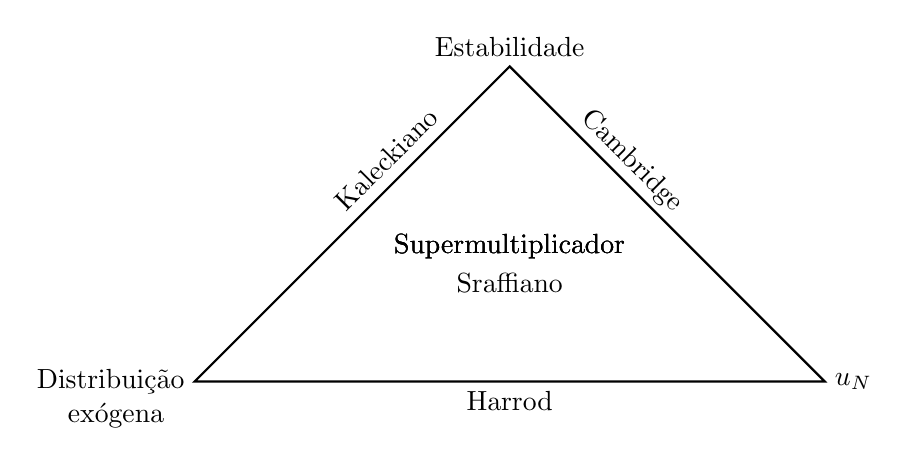
\begin{tikzpicture}[thick]
    \path[draw] (-4,0)  coordinate [label= left:Distribuição] (A)

            -- ( 0,4)  coordinate [label=above:Estabilidade] (C)
            -- ( 4,0)  coordinate [label=right:$u_N$] (B)
            -- cycle;
    \foreach \point in {A,B,C}
    \draw
        -- (0,2) node[anchor=north]{Supermultiplicador};
    \draw
        -- (-5,-0.15) node[anchor=north]{exógena};
    \draw
        -- (0,1.5) node[anchor=north]{Sraffiano};
    \draw
        -- (-1.75,3) node[anchor=north, rotate=45]{Kaleckiano};
    \draw
        -- (1.75,3) node[anchor=north, rotate=-45]{Cambridge};
    \draw
        -- (0,0) node[anchor=north]{Harrod};
\end{tikzpicture}
}
\end{center}
\caption*{\textbf{Fonte:} Elaboração própria}
\end{figure}
\noindent Essa trindade impossível se mostrou falsa com o desenvolvimento do supermultiplicador sraffiano, proposto por \textcite{serrano_long_1995} e \textcite{bortis_institutions_1996}. Portanto, diante da discussão anterior, conclui-se que o modelo do SSM não é incompatível para analisar o médio prazo ou restrito ao longo prazo como afirma \textcite{nikiforos_comments_2018}. Com isso, encerra-se este capítulo elegendo o supermultiplicador sraffiano como o mais adequado por replicar os fatos estilizados mencionados anteriormente e por validar o PDE no curto, médio e longo prazo. Seguindo a sugestão de \textcite[p.~280]{freitas_growth_2015}, esta investigação avança no sentido de contribuir para a compreensção de outros componentes da demanda agregada não criadores de capacidade. Destaca-se ainda que a instabilidade da economia não decorre da junção do acelerador com o multiplicador\footnote{Como mostram \textcite{serrano_trouble_2017}, dadas certas condições, o SSM é dinamicamente \textit{estável}.}, mas sim da própria instabilidade da demanda agregada \cite{dejuan_hidden_2017}.  Dito isso,  o capítulo seguinte irá esboçar alguns esforços para evidenciar a importância do investimento residencial para a dinâmica do ciclo econômico norte americano e, assim, preencher uma das lacunas dos modelos de crescimento com gastos autônomos.









\begin{comment}
mais especificamente:
\begin{itemize}
\item \textbf{Curto-prazo:} Determinação da poupança pelo investimento \cite{keynes_general_1936};
\item \textbf{Médio-prazo:} Relação positiva entre taxa de investimento e crescimento \cite{cesaratto_neo-kaleckian_2015};
\item \textbf{Longo-prazo:} Convergência ao grau de utilização ao normal\footnote{Por grau de utilização normal, adota-se a definição de \textcites[p.~423--4, Original de 1986]{ciccone_2017}: ``\textit{The `normal' utilization of capacity can therefore imply not only the expectation of a certain breadth and frequency of the fluctuations in demand, but also the expectation of the idleness of the excess capacity deliberately chosen by the entrepreneurs;}'' } \cites{ciccone_2017}{vianello_pace_1985}.
\end{itemize}
\end{comment}